% A LaTeX template for MSc Thesis submissions to 
% Politecnico di Milano (PoliMi) - School of Industrial and Information Engineering
%
% S. Bonetti, A. Gruttadauria, G. Mescolini, A. Zingaro
% e-mail: template-tesi-ingind@polimi.it
%
% Last Revision: October 2021
%
% Copyright 2021 Politecnico di Milano, Italy. NC-BY

\documentclass{Configuration_Files/PoliMi3i_thesis}

%------------------------------------------------------------------------------
%	REQUIRED PACKAGES AND  CONFIGURATIONS
%------------------------------------------------------------------------------

% CONFIGURATIONS
\usepackage{parskip} % For paragraph layout
\usepackage{setspace} % For using single or double spacing
\usepackage{emptypage} % To insert empty pages
\usepackage{multicol} % To write in multiple columns (executive summary)
\setlength\columnsep{15pt} % Column separation in executive summary
\setlength\parindent{0pt} % Indentation
\raggedbottom  

% PACKAGES FOR TITLES
\usepackage{titlesec}
% \titlespacing{\section}{left spacing}{before spacing}{after spacing}
\titlespacing{\section}{0pt}{3.3ex}{2ex}
\titlespacing{\subsection}{0pt}{3.3ex}{1.65ex}
\titlespacing{\subsubsection}{0pt}{3.3ex}{1ex}
\usepackage{color}

% PACKAGES FOR LANGUAGE AND FONT
\usepackage[english]{babel} % The document is in English  
\usepackage[utf8]{inputenc} % UTF8 encoding
\usepackage[T1]{fontenc} % Font encoding
\usepackage[11pt]{moresize} % Big fonts

% PACKAGES FOR IMAGES
\usepackage{graphicx}
\usepackage{transparent} % Enables transparent images
\usepackage{eso-pic} % For the background picture on the title page
\usepackage{subfig} % Numbered and caption subfigures using \subfloat.
\usepackage{tikz} % A package for high-quality hand-made figures.
\usetikzlibrary{}
\graphicspath{{./Images/}} % Directory of the images
\usepackage{caption} % Coloured captions
\usepackage{xcolor} % Coloured captions
\usepackage{amsthm,thmtools,xcolor} % Coloured "Theorem"
\usepackage{float}

% STANDARD MATH PACKAGES
\usepackage{amsmath}
\usepackage{amsthm}
\usepackage{amssymb}
\usepackage{amsfonts}
\usepackage{bm}
\usepackage[overload]{empheq} % For braced-style systems of equations.
\usepackage{fix-cm} % To override original LaTeX restrictions on sizes

% PACKAGES FOR TABLES
\usepackage{tabularx}
\usepackage{longtable} % Tables that can span several pages
\usepackage{colortbl}

% PACKAGES FOR ALGORITHMS (PSEUDO-CODE)
\usepackage{algorithm}
\usepackage{algorithmic}

% PACKAGES FOR REFERENCES & BIBLIOGRAPHY
\usepackage[colorlinks=true,linkcolor=black,anchorcolor=black,citecolor=black,filecolor=black,menucolor=black,runcolor=black,urlcolor=black]{hyperref} % Adds clickable links at references
\usepackage{cleveref}
\usepackage[square, numbers, sort&compress]{natbib} % Square brackets, citing references with numbers, citations sorted by appearance in the text and compressed
\bibliographystyle{abbrvnat} % You may use a different style adapted to your field

% OTHER PACKAGES
\usepackage{pdfpages} % To include a pdf file
\usepackage{afterpage}
\usepackage{lipsum} % DUMMY PACKAGE
\usepackage{fancyhdr} % For the headers
\fancyhf{}

% Input of configuration file. Do not change config.tex file unless you really know what you are doing. 
% Define blue color typical of polimi
\definecolor{bluepoli}{cmyk}{0.4,0.1,0,0.4}

% Custom theorem environments
\declaretheoremstyle[
  headfont=\color{bluepoli}\normalfont\bfseries,
  bodyfont=\color{black}\normalfont\itshape,
]{colored}

% Set-up caption colors
\captionsetup[figure]{labelfont={color=bluepoli}} % Set colour of the captions
\captionsetup[table]{labelfont={color=bluepoli}} % Set colour of the captions
\captionsetup[algorithm]{labelfont={color=bluepoli}} % Set colour of the captions

\theoremstyle{colored}
\newtheorem{theorem}{Theorem}[chapter]
\newtheorem{proposition}{Proposition}[chapter]

% Enhances the features of the standard "table" and "tabular" environments.
\newcommand\T{\rule{0pt}{2.6ex}}
\newcommand\B{\rule[-1.2ex]{0pt}{0pt}}

% Pseudo-code algorithm descriptions.
\newcounter{algsubstate}
\renewcommand{\thealgsubstate}{\alph{algsubstate}}
\newenvironment{algsubstates}
  {\setcounter{algsubstate}{0}%
   \renewcommand{\STATE}{%
     \stepcounter{algsubstate}%
     \Statex {\small\thealgsubstate:}\space}}
  {}

% New font size
\newcommand\numfontsize{\@setfontsize\Huge{200}{60}}

% Title format: chapter
\titleformat{\chapter}[hang]{
\fontsize{50}{20}\selectfont\bfseries\filright}{\textcolor{bluepoli} \thechapter\hsp\hspace{2mm}\textcolor{bluepoli}{|   }\hsp}{0pt}{\huge\bfseries \textcolor{bluepoli}
}

% Title format: section
\titleformat{\section}
{\color{bluepoli}\normalfont\Large\bfseries}
{\color{bluepoli}\thesection.}{1em}{}

% Title format: subsection
\titleformat{\subsection}
{\color{bluepoli}\normalfont\large\bfseries}
{\color{bluepoli}\thesubsection.}{1em}{}

% Title format: subsubsection
\titleformat{\subsubsection}
{\color{bluepoli}\normalfont\large\bfseries}
{\color{bluepoli}\thesubsubsection.}{1em}{}

% Shortening for setting no horizontal-spacing
\newcommand{\hsp}{\hspace{0pt}}

\makeatletter
% Renewcommand: cleardoublepage including the background pic
\renewcommand*\cleardoublepage{%
  \clearpage\if@twoside\ifodd\c@page\else
  \null
  \AddToShipoutPicture*{\BackgroundPic}
  \thispagestyle{empty}%
  \newpage
  \if@twocolumn\hbox{}\newpage\fi\fi\fi}
\makeatother

%For correctly numbering algorithms
\numberwithin{algorithm}{chapter}

%----------------------------------------------------------------------------
%	NEW COMMANDS DEFINED
%----------------------------------------------------------------------------

% EXAMPLES OF NEW COMMANDS
\newcommand{\bea}{\begin{eqnarray}} % Shortcut for equation arrays
\newcommand{\eea}{\end{eqnarray}}
\newcommand{\e}[1]{\times 10^{#1}}  % Powers of 10 notation

%----------------------------------------------------------------------------
%	ADD YOUR PACKAGES (be careful of package interaction)
%----------------------------------------------------------------------------

%----------------------------------------------------------------------------
%	ADD YOUR DEFINITIONS AND COMMANDS (be careful of existing commands)
%----------------------------------------------------------------------------

% Placeholder marker for results still to be filled in (remove when the text is final)
\providecommand{\tbd}[1]{\textcolor{red}{[#1]}}

%----------------------------------------------------------------------------
%	BEGIN OF YOUR DOCUMENT
%----------------------------------------------------------------------------

\begin{document}

\fancypagestyle{plain}{%
\fancyhf{} % Clear all header and footer fields
\fancyhead[RO,RE]{\thepage} %RO=right odd, RE=right even
\renewcommand{\headrulewidth}{0pt}
\renewcommand{\footrulewidth}{0pt}}

%----------------------------------------------------------------------------
%	TITLE PAGE
%----------------------------------------------------------------------------

\pagestyle{empty} % No page numbers
\frontmatter % Use roman page numbering style (i, ii, iii, iv...) for the preamble pages

\puttitle{
	title=Geotechnical Behaviour of Icy-Lunar Regolith, % Title of the thesis
	name=Leonardo Sacco, % Author Name and Surname
	course=Geotechnical Engineering - Ingegneria Geotecnica, % Study Programme (in Italian)
	ID  = 280654,  % Student ID number (numero di matricola)
	advisor= Prof. Nicola Cefis, % Supervisor name
	coadvisor={Christine McCarthy, Marco Caruso}, % Co-Supervisor name, remove this line if there is none
	academicyear={2026-27},  % Academic Year
} % These info will be put into your Title page 

%----------------------------------------------------------------------------
%	PREAMBLE PAGES: ABSTRACT (inglese e italiano), EXECUTIVE SUMMARY
%----------------------------------------------------------------------------
\startpreamble
\setcounter{page}{1} % Set page counter to 1

% ABSTRACT IN ENGLISH
% Passages wrapped in \tbd{...} are placeholders: replace them with the actual results, then remove the macro.
\chapter*{Abstract}
Water ice mixed with regolith in the permanently shadowed regions of the Moon is a prime target for in-situ resource utilisation, yet the time-dependent mechanical behaviour of icy lunar regolith remains poorly constrained. Existing data consist mainly of strength measurements on ice-cemented simulants, and almost no creep data exist for confined, granular ice--regolith mixtures at low temperature. This thesis addresses that gap through laboratory experiments and constitutive modelling.

Mixtures of granular water ice (250--500~$\mu$m) and the lunar highlands simulant LHS-1 were tested in a uniaxial (oedometric) compaction vessel adapted for sub-freezing operation, at temperatures between $-10$ and $-40~^{\circ}$C and axial stresses up to about 3~MPa. Ice content and temperature were varied systematically, and the results were compared with pure-ice data from the same apparatus. Piston seal friction, system compliance and the usable displacement range were quantified through calibration tests, and the applied stress was corrected accordingly. \tbd{Seal friction was found to be of the order of 0.2--0.4~MPa during sliding and up to about 1.3~MPa at breakaway.}

\tbd{Sample height decreased approximately linearly with the logarithm of time under constant stress. Compaction rates decreased with decreasing temperature and with increasing regolith fraction, with an apparent activation energy of \ldots~kJ/mol and a stress exponent of \ldots.} \tbd{A transition from ice-dominated to skeleton-dominated behaviour was observed at an ice content of about \ldots~wt\%.}

The results were used to calibrate a densification law in which the compaction rate follows a power law in stress and an Arrhenius dependence on temperature, and varies with porosity and ice fraction. The law is suitable for finite-element implementation with temperature as an input field. The limitations of the oedometric configuration (unmeasured radial stress, wall friction) and of the extrapolation to lunar cryogenic temperatures are discussed.
\\
\\
\textbf{Keywords:} lunar regolith, water ice, creep, oedometric compaction, constitutive modelling, in-situ resource utilisation % Keywords

% ABSTRACT IN ITALIAN
\chapter*{Abstract in lingua italiana}
Il ghiaccio d'acqua mescolato alla regolite nelle regioni lunari permanentemente in ombra è una risorsa promettente per l'utilizzo in situ, ma il comportamento meccanico nel tempo della regolite ghiacciata è ancora poco noto. I dati disponibili riguardano soprattutto la resistenza di simulanti cementati dal ghiaccio, e mancano quasi del tutto dati di creep su miscele granulari confinate a bassa temperatura. Questa tesi affronta tale lacuna con prove di laboratorio e modellazione costitutiva.

Miscele di ghiaccio granulare (250--500~$\mu$m) e del simulante lunare LHS-1 sono state provate in una cella di compattazione uniassiale (edometrica) adattata alle basse temperature, tra $-10$ e $-40~^{\circ}$C e con sforzi assiali fino a circa 3~MPa. Contenuto di ghiaccio e temperatura sono stati variati in modo sistematico, e i risultati confrontati con dati sul solo ghiaccio ottenuti con lo stesso apparato. Attrito delle guarnizioni del pistone, cedevolezza del sistema e campo utile di misura dello spostamento sono stati quantificati con prove di taratura, e lo sforzo applicato è stato corretto di conseguenza. \tbd{L'attrito delle guarnizioni vale 0.2--0.4~MPa in scorrimento e fino a circa 1.3~MPa al primo distacco.}

\tbd{Sotto sforzo costante l'altezza dei provini cala in modo circa lineare con il logaritmo del tempo. La velocità di compattazione cala con la temperatura e al crescere della frazione di regolite, con un'energia di attivazione apparente di \ldots~kJ/mol e un esponente dello sforzo pari a \ldots.} \tbd{La transizione da un comportamento dominato dal ghiaccio a uno dominato dallo scheletro solido avviene intorno al \ldots~\% in massa di ghiaccio.}

I risultati sono serviti a calibrare una legge di densificazione in cui la velocità di compattazione segue una legge di potenza nello sforzo e una dipendenza di Arrhenius dalla temperatura, e varia con porosità e frazione di ghiaccio. La legge è implementabile agli elementi finiti con la temperatura come campo in ingresso. Si discutono i limiti della prova edometrica (sforzo radiale non misurato, attrito sulla parete) e dell'estrapolazione alle temperature lunari.
\\
\\
\textbf{Parole chiave:} regolite lunare, ghiaccio d'acqua, creep, compattazione edometrica, modellazione costitutiva, utilizzo delle risorse in situ % Keywords (italian)

%----------------------------------------------------------------------------
%	LIST OF CONTENTS/FIGURES/TABLES/SYMBOLS
%----------------------------------------------------------------------------

% TABLE OF CONTENTS
\thispagestyle{empty}
\tableofcontents % Table of contents 
\thispagestyle{empty}
\cleardoublepage

%-------------------------------------------------------------------------
%	THESIS MAIN TEXT
%-------------------------------------------------------------------------
% In the main text of your thesis you can write the chapters in two different ways:
%
%(1) As presented in this template you can write:
%    \chapter{Title of the chapter}
%    *body of the chapter*
%
%(2) You can write your chapter in a separated .tex file and then include it in the main file with the following command:
%    \chapter{Title of the chapter}
%    \input{chapter_file.tex}
%
% Especially for long thesis, we recommend you the second option.

\addtocontents{toc}{\vspace{2em}} % Add a gap in the Contents, for aesthetics
\mainmatter % Begin numeric (1,2,3...) page numbering

% --------------------------------------------------------------------------
% NUMBERED CHAPTERS % Regular chapters following
% --------------------------------------------------------------------------
\chapter*{Introduction}
\label{ch:introduction}%
% ---------------------------------------------------------------------------
% INTRODUCTION (unnumbered)
% Aim: 3-5 pages. Why the problem matters, what is missing, what this thesis does.
% ---------------------------------------------------------------------------

\section*{Motivation}

Over the last three decades, orbital and impact measurements have shown that the polar regions of the Moon contain water ice. Neutron spectrometers detected hydrogen enrichment at both poles~\cite{feldman1998,mitrofanov2010}. The LCROSS impact into the permanently shadowed crater Cabeus excavated regolith containing about 5.6\,wt\% of water ice~\cite{colaprete2010}, and near-infrared spectra revealed ice exposed at the surface of the coldest polar craters~\cite{li2018}. This ice is stored in permanently shadowed regions and in the shallow subsurface of the polar terrains, where temperatures stay between about 40 and 110\,K~\cite{paige2010,williams2019}.

Water is the most valuable resource on the Moon. It can provide drinking water and oxygen for crews and, split into hydrogen and oxygen, rocket propellant. For this reason, the main lunar exploration programmes plan to land near the south pole and to extract ice in situ (in-situ resource utilisation, ISRU). Every step of this activity depends on how icy regolith deforms:
\begin{itemize}
    \item excavators and drills must break and remove it;
    \item rovers and landing pads load its surface;
    \item habitats, processing plants and antennas need foundations that will rest on it, or in it, for years.
\end{itemize}
In the low lunar gravity, the overburden stress, and therefore the confinement of the soil, is about one sixth of that at the same depth on Earth. Foundations and anchors will have to reach deeper to find adequate support, and are likely to meet ice-bearing layers.

Ice creeps. At any temperature above absolute zero and under any sustained stress, it deforms with time, at a rate that increases steeply with stress and temperature~\cite{glen1955,goldsby2001}. A structure resting on icy regolith will therefore keep settling after construction. The heat released by a habitat or a processing plant will warm the ground and accelerate this creep. Designing for these conditions requires a description of how icy regolith compacts and creeps over time, as a function of stress, temperature and ice content. Strength alone is not enough.

\section*{Problem statement}

Most mechanical data on icy lunar simulants come from strength tests designed to assess excavation: unconfined compression, indentation and cone penetration tests~\cite{gertsch2006,pitcher2016,atkinson2020,liu2022,ricardo2026}. These tests share three features that limit their use for the problem above.
\begin{enumerate}
    \item \textbf{Ice morphology.} Most samples are ice-cemented: liquid water is mixed with the simulant and frozen. On the Moon liquid water is not stable, and ice was most likely deposited from vapour and then mixed with the regolith by impacts~\cite{cannon2020}. The morphology of the ice changes the strength by orders of magnitude at the same ice content~\cite{ricardo2026}, so data on ice-cemented samples cannot be transferred directly to lunar conditions.
    \item \textbf{Time dependence.} Strength is measured at a single rate. The time-dependent behaviour, which controls the long-term settlement of structures, has been measured only in a few relaxation tests~\cite{atkinson2020}.
    \item \textbf{Confinement.} Almost all tests are unconfined. Below the surface, the soil is laterally confined, and its behaviour under one-dimensional (oedometric) compression is the reference for settlement analyses.
\end{enumerate}
The large body of knowledge on terrestrial frozen soils does not fill this gap. It concerns mostly saturated, ice-cemented soils close to $0\,^\circ$C, where unfrozen water dominates the response~\cite{andersland2004,arenson2007}. The densification of granular ice under constant stress is well understood for polar snow and firn~\cite{herron1980,arnaud2000}, but it has not been studied in mixtures with lunar regolith. As a result, there are no oedometric creep or compaction data on granular ice--regolith mixtures at low temperature, and no calibrated law that describes their time-dependent compaction as a function of stress, temperature, porosity and ice content.

\section*{Objectives}

This thesis addresses the gap with laboratory compaction tests on granular mixtures of ice and the lunar highlands simulant LHS-1. The work was carried out at the Lamont--Doherty Earth Observatory of Columbia University, in a laboratory that had previously used the same compaction vessel to study the densification of synthetic firn~\cite{skarbek2025data}. The objectives are three.
\begin{enumerate}
    \item \textbf{Bring a low-temperature uniaxial compaction vessel into operation and characterise it.} The vessel applies a constant axial stress through a pressurised oil chamber and a piston, under rigid lateral confinement, at temperatures down to $-40\,^\circ$C. Before it can give reliable data on a new material, the losses between the oil pressure and the stress on the sample (seal friction), the compliance of the oil circuit, the range of the displacement transducer and the thermal drift must be measured, and a test procedure must be defined.
    \item \textbf{Measure the compaction of ice--regolith mixtures} as a function of axial stress, temperature and ice content, from the initial loose state through the time-dependent densification under constant stress. The results are expressed in the soil-mechanics framework of void ratio, compression index and coefficient of secondary compression, so that they can be compared with both granular ice and frozen soils.
    \item \textbf{Calibrate a temperature-dependent densification law} usable in numerical analyses. The law relates the compaction rate to stress through a power law and to temperature through an Arrhenius term, and lets it depend on porosity and ice content. It is formulated so that it can be implemented in a finite element code with temperature as an input field.
\end{enumerate}

\section*{Scope and limitations}

The scope of the work is limited in the following ways.
\begin{itemize}
    \item \textbf{Oedometric conditions only.} The vessel imposes zero lateral strain and measures only the axial stress. The radial stress is not measured, so the results describe one-dimensional compression and not the full three-dimensional behaviour. Friction between the sample and the chamber wall reduces the stress towards the bottom of the sample. It is minimised but not eliminated, and its effect is discussed in Chapter~\ref{ch:characterisation}.
    \item \textbf{Laboratory temperatures.} The tests are carried out between $-10$ and $-40\,^\circ$C, much warmer than the lunar polar subsurface ($-235$ to $-165\,^\circ$C). The results apply to lunar conditions only through the temperature dependence of the calibrated law. The extrapolation is physically motivated, because the creep of ice remains thermally activated down to cryogenic temperatures~\cite{durham1997}, but it carries an uncertainty that cannot be removed with the present apparatus.
    \item \textbf{One simulant and one ice morphology.} Only LHS-1 is used, as representative of the highland terrains that surround the lunar poles. The ice is granular: crushed, sieved and mixed dry with the simulant. During compaction the mixture evolves towards a pressure-sintered state. Vapour-deposited and ice-cemented morphologies are not studied. Since granular mixtures are among the weakest, the results are expected to be conservative for design.
    \item \textbf{Stresses and durations.} The axial stress is limited to 3.4\,MPa by the pressure controller, and each test lasts from one to a few days. These stresses cover the range of foundation and equipment loads near the surface, but the long-term behaviour over the lifetime of a structure is obtained by extrapolating the log-time compaction observed in the laboratory.
    \item \textbf{Number of tests.} The experimental campaign was carried out within a limited period, and each test occupies the vessel for one to several days. The test programme was therefore designed to vary one parameter at a time, with few repetitions.
\end{itemize}

\section*{Outline of the thesis}

Chapter~\ref{ch:background} reviews the state of the art: the evidence for lunar polar ice and its likely morphology, the properties of lunar regolith and of LHS-1, the rheology of ice with and without particles, the densification of granular ice, the creep of frozen soils with the constitutive models that describe it, and the existing mechanical tests on icy simulants. It closes by defining the research gap.

Chapter~\ref{ch:materials_apparatus} describes the materials (LHS-1, granular ice and their mixtures) and the experimental apparatus: the uniaxial compaction vessel, its loading, displacement-measurement and temperature-control systems, and the data acquisition.

Chapter~\ref{ch:characterisation} presents the characterisation of the apparatus (seal friction, compliance of the oil circuit, range of the displacement transducer, thermal drift and wall friction) and the resulting test procedure and data reduction, including the calculation of the void ratio from the oil volume when the transducer is out of range.

Chapter~\ref{ch:results} reports the results of the compaction tests on pure ice, on dry LHS-1 and on the mixtures, including unloading--reloading stages and post-test measurements, and discusses the effects of stress, temperature and ice content.

Chapter~\ref{ch:modelling} formulates the densification law, calibrates its parameters on the experimental data, compares it with the measurements and discusses its implementation in a finite element code and its implications for lunar engineering.

Chapter~\ref{ch:conclusions} summarises the main findings and gives recommendations for future work. Appendix~\ref{app:protocol} contains the detailed test protocol and Appendix~\ref{app:tests} the log of all the tests carried out, with the calibration data of the apparatus.

\chapter{Background and state of the art}
\label{ch:background}%
% Aim: 20-25 pages. Everything the reader needs to judge Chapters 3-5. End with the gap this thesis fills.

This chapter collects the knowledge needed to design, run and interpret the experiments of this thesis. It moves from the lunar setting (where the ice is, how cold it is and in what form it is likely to occur) to the materials (the regolith, its simulant LHS-1 and ice), and then to the mechanics: the creep of ice, the densification of granular ice, the creep of frozen soils and the constitutive models that describe it. The chapter closes with the few mechanical data that exist on icy lunar simulants and with the gap that this work addresses. Only the lunar highlands simulant LHS-1 is used in this thesis, and the review of simulant properties is restricted to it.

% ---------------------------------------------------------------------------
\section{Water ice on the Moon}
\label{sec:lunar_ice}
% ---------------------------------------------------------------------------

\subsection{Evidence for polar ice}

The Moon's spin axis is tilted by only about $1.5^\circ$ to the ecliptic. As a result, the floors of many craters near the poles never receive direct sunlight. These permanently shadowed regions (PSRs) are among the coldest surfaces in the Solar System and act as cold traps: water molecules that reach them, whether delivered by comets and asteroids, produced by the solar wind or released from the interior, can stay there for geological times~\cite{vasavada1999,lucey2022}.

Several independent measurements point to water ice in and around these cold traps:
\begin{itemize}
    \item \textbf{Neutron spectroscopy.} Lunar Prospector measured a deficit of epithermal neutrons of 4.6\% over the north pole and 3.0\% over the south pole, interpreted as hydrogen, most plausibly water ice buried under up to about 40\,cm of dry regolith~\cite{feldman1998,feldman2001}. The Lunar Exploration Neutron Detector (LEND) on the Lunar Reconnaissance Orbiter (LRO) refined these maps and gave 0.5--4.0\,wt\% of water ice at the site later hit by LCROSS, depending on the thickness of the dry cover. Several hydrogen-rich areas do not coincide with PSRs~\cite{mitrofanov2010}.
    \item \textbf{Impact experiment.} In 2009 the LCROSS mission impacted a spent rocket stage into the PSR of Cabeus crater. The ejecta plume contained about $155\pm12$\,kg of water vapour and ice, corresponding to $5.6\pm2.9$\,wt\% of water ice in the regolith, together with other volatiles such as H$_2$S, CO$_2$ and light hydrocarbons~\cite{colaprete2010}.
    \item \textbf{Surface spectroscopy.} Near-infrared spectra from the Moon Mineralogy Mapper (M$^3$) gave direct evidence of ice exposed at the surface within $20^\circ$ of both poles, only where the annual maximum temperature stays below about 110\,K. Exposed ice was found in only about 3.5\% of the cold traps, and some pixels may contain up to about 30\,wt\% ice~\cite{li2018}. Ultraviolet albedo and temperature data from LRO support patchy surface frost in the south polar region~\cite{hayne2015}.
\end{itemize}

\subsection{Thermal environment}

The Diviner radiometer on LRO showed that cold-trapping conditions extend beyond the permanently shadowed areas and that, in some craters, temperatures stay below 40\,K throughout the year; the subsurface temperature at the LCROSS impact site was estimated at about 38\,K~\cite{paige2010}. In winter, the area that stays below 110\,K, the commonly used threshold for long-term ice stability, grows by factors of 2.8 in the south and 4.3 in the north~\cite{williams2019}.

Below the surface, the daily and seasonal temperature waves are damped within a few tens of centimetres to about a metre, and the temperature tends to a nearly constant value set by the mean surface energy balance and the internal heat flux. This deep value depends strongly on latitude and local shadowing:
\begin{itemize}
    \item at the Apollo~15 and~17 sites (about $26^\circ$N and $20^\circ$N), the heat-flow probes measured $252\pm5$\,K ($-21\,^\circ$C) at 0.83\,m and $256\pm5$\,K ($-17\,^\circ$C) at 1.3\,m~\cite{langseth1976,hayne2017};
    \item on flat terrain at the poles, models give a stable subsurface temperature of about 93\,K ($-180\,^\circ$C)~\cite{vasavada1999};
    \item inside PSRs the subsurface stays between about 40 and 110\,K ($-235$ to $-165\,^\circ$C)~\cite{paige2010,williams2019}.
\end{itemize}
The value of about $-20\,^\circ$C, often quoted for the lunar subsurface, therefore applies to equatorial and mid-latitude sites. At the polar sites where ice is expected, the ground is more than 100\,K colder. This has two consequences for this thesis. First, the laboratory temperatures used here ($-10$ to $-40\,^\circ$C) are far warmer than the lunar polar subsurface, and the results must be extrapolated with a temperature-dependent law (Sections~\ref{sec:ice_rheology} and~\ref{sec:frozen_soils}). Second, the large temperature gradients near PSR boundaries, and the heat that structures and processing plants would introduce, mean that icy regolith around a lunar installation will not be at a single temperature. A constitutive law with temperature as an explicit input is required.

\subsection{Why the time-dependent behaviour matters}

Water ice is the main target of in-situ resource utilisation (ISRU) on the Moon: it can provide drinking water, oxygen and hydrogen propellant. Extracting it requires excavation, drilling, trafficking and the foundation of plants and habitats on or in ice-bearing ground. The low lunar gravity ($1.62$\,m/s$^2$, about one sixth of Earth's) gives low overburden stresses and therefore little confinement near the surface; to obtain adequate bearing capacity and anchorage, foundations and piles are likely to reach depths where buried ice may be present. Under a sustained load, ice creeps at any stress, and a mixture of ice and regolith will continue to settle over the lifetime of a structure. Strength alone, which is what most existing tests on icy simulants measure (Section~\ref{sec:icy_regolith_data}), does not describe this behaviour.

\subsection{Expected ice contents}

Estimates of the ice content of polar regolith span more than an order of magnitude: below 1\,wt\% from orbital neutron data averaged over large footprints, about 1--4\,wt\% from LEND, $5.6\pm2.9$\,wt\% from the single LCROSS sample, and up to about 30\,wt\% in exposed surface patches~\cite{feldman2001,mitrofanov2010,colaprete2010,li2018}. Models of ice delivery and impact gardening predict a strongly layered and laterally variable distribution~\cite{cannon2020,cannonbritt2020}. In this thesis, ice contents in the range of a few to a few tens of percent by mass are therefore considered realistic, and the definition of ice content must always be stated, as discussed in Section~\ref{subsec:ice_content_def}.

\subsection{Ice morphology in regolith}
\label{subsec:morphology}

The way ice is arranged among the regolith grains, its morphology, is at least as important as its amount. Four idealised morphologies are used in the literature on icy simulants~\cite{johnson2024,ricardo2026}:
\begin{itemize}
    \item \textbf{ice-cemented}: liquid water is mixed with the soil and frozen, so that ice fills the pores and bonds the grains, as in terrestrial permafrost;
    \item \textbf{granular} (or unsintered): ice particles are mixed with dry regolith grains, with little or no bonding between them;
    \item \textbf{pressure-sintered}: a granular mixture is compacted so that ice grains bond to each other and to the regolith at their contacts;
    \item \textbf{vapour-deposited}: water vapour condenses directly on cold regolith grains, forming coatings and necks between them.
\end{itemize}

On the Moon, liquid water is not stable at the surface: in the absence of an atmosphere, ice sublimates without melting. Ice is therefore thought to have been emplaced mainly by condensation of vapour in cold traps, and then mixed, buried and redistributed by impacts. Models of this process predict ice-rich layers buried under younger, ice-poor ejecta, and deposits that are reworked into mixtures of ice and regolith fragments~\cite{cannon2020,cannonbritt2020}. Pore-filling ice cemented by a liquid phase, the usual morphology in terrestrial permafrost and the easiest to make in the laboratory, is unlikely to be representative of lunar conditions.

The mechanical consequences are large. In the only single-laboratory study of all four morphologies, carried out on LHS-1 at about $-180\,^\circ$C with cone penetration tests, ice-cemented samples were several orders of magnitude stronger than the others. A vapour-deposited sample with 6.88\,wt\% ice was 3.92 times stronger than a pressure-sintered sample with 8\,wt\% ice~\cite{ricardo2026}. The specific energy for excavation rose from 2.74 to 143\,J/g between 1 and 12\,wt\% ice for ice-cemented samples, whereas it stayed below 0.4\,J/g for pressure-sintered ones~\cite{ricardo2026}.

This thesis studies \textbf{granular mixtures}: ice crushed and sieved to a grain size comparable to that of the coarser regolith fraction, mixed with dry LHS-1 and compacted in the test itself. During the test the mixture evolves from an unbonded granular state towards a pressure-sintered one. Among the four morphologies, this is the weakest and closest to the reworked, gardened deposits expected in the upper metres of polar regolith. Results obtained on granular mixtures are therefore expected to be conservative, that is, to give more deformation and less strength than vapour-deposited or ice-cemented material with the same ice content.

\subsection{Defining the ice content}
\label{subsec:ice_content_def}

Studies on icy soils use different definitions of ice content, and much of the apparent disagreement between them comes from this. With $m_i$ and $m_s$ the masses of ice and dry soil, $\rho_i = 0.917$\,g/cm$^3$ the density of ice and $\rho_s$ the grain density of the soil, the following quantities are used in this thesis:
\begin{align}
    w_i &= \frac{m_i}{m_s} && \text{(gravimetric ice content, geotechnical convention, ``wt\% dry'')},\label{eq:wi}\\
    x_i &= \frac{m_i}{m_i+m_s} && \text{(mass fraction of ice in the solids)},\label{eq:xi}\\
    \phi_s &= \frac{m_s/\rho_s}{m_s/\rho_s + m_i/\rho_i} && \text{(volume fraction of soil in the solid phases)},\label{eq:phis}\\
    S_i &= \frac{V_i}{V_v} = \frac{w_i\,\rho_s}{e_s\,\rho_i} && \text{(ice saturation of the soil pores)},\label{eq:Si}
\end{align}
where $V_i$ is the volume of ice, $V_v$ the volume of pores between the soil grains and $e_s$ the void ratio of the soil skeleton alone. Remote-sensing results are usually expressed as $x_i$, geotechnical studies as $w_i$; the two differ by about 10\% of their value at $w_i = 10$\,wt\% and by 30\% at $w_i = 40$\,wt\%.

Equation~\eqref{eq:Si} shows when ice stops being a pore filler. For LHS-1 at a dry density of 1.5\,g/cm$^3$ ($e_s\approx0.83$ with $\rho_s = 2.75$\,g/cm$^3$), the pores are completely filled at $w_i\approx28$\,wt\%. Above this value the mixture is \emph{ice-rich}: the soil grains are no longer in contact, they are suspended in the ice, and the mechanical behaviour is controlled by the ice matrix rather than by the soil skeleton~\cite{ting1983,arenson2007}. The local ice contents of up to 30\,wt\% inferred from M$^3$ data~\cite{li2018} fall at this transition.

% ---------------------------------------------------------------------------
\section{Lunar regolith and its simulants}
\label{sec:regolith}
% ---------------------------------------------------------------------------

\subsection{Lunar regolith}

The lunar regolith is the layer of fragmented, unconsolidated material that covers the bedrock. It is several metres thick, and thicker on the older highlands than on the maria. It has been produced by billions of years of meteorite impacts, which break, melt and weld the rock. Without an atmosphere or liquid water there is no chemical weathering, transport or sorting by wind or water, so the grains are not rounded: lunar soil particles are irregular, angular to subangular and often elongated, with re-entrant surfaces. A large fraction consists of agglutinates, aggregates of mineral and glass fragments bonded by impact-melt glass~\cite{carrier1991}.

The geotechnical properties of the returned Apollo and Luna samples, and of the in-situ measurements, are summarised by Carrier et al.~\cite{carrier1991}:
\begin{itemize}
    \item median grain size between 40 and 130\,$\mu$m, on average about 70\,$\mu$m: the soil is a well-graded silty sand;
    \item specific gravity of the grains of about 3.1, with a range from 2.3 to above 3.2 depending on mineralogy and on the porosity of agglutinates;
    \item bulk density of $1.50\pm0.05$\,g/cm$^3$ in the top 15\,cm and $1.66\pm0.05$\,g/cm$^3$ in the top 60\,cm, increasing towards about 1.9\,g/cm$^3$ at depth;
    \item porosity of about 49\% in the top 30\,cm and relative density of about 65\% in the top 15\,cm, rising above 90\% below 30\,cm. Below a few tens of centimetres, the regolith is very dense.
\end{itemize}

The two main terrains, mare and highlands, differ in composition. The maria are basaltic lava plains rich in pyroxene, olivine and ilmenite. The highlands, which cover most of the lunar surface including the polar regions, are dominated by anorthosite, a rock made mostly of calcium-rich plagioclase feldspar. A highlands simulant is therefore the appropriate choice for the polar regions where ice is expected.

\subsection{The LHS-1 simulant}

Returned lunar samples are too scarce and valuable for destructive geotechnical testing, and research relies on simulants that reproduce some of their properties. LHS-1 (Lunar Highlands Simulant) is produced by Exolith Lab, a spin-off of the University of Central Florida, from terrestrial anorthosite and glass-rich basalt, crushed and blended to approximate the mineralogy and grain size distribution of lunar highland soils~\cite{isachenkov2022,exolithLHS1}. Its main properties are listed in Table~\ref{tab:lhs1}.

\begin{table}[H]
    \centering
    \caption{Properties of the LHS-1 lunar highlands simulant. Values from the manufacturer's specification sheet (batch of December 2022)~\cite{exolithLHS1} unless otherwise stated. Properties vary between production batches; the batch used in this work is described in Chapter~\ref{ch:materials_apparatus}.}
    \label{tab:lhs1}
    \begin{tabularx}{\textwidth}{|>{\raggedright\arraybackslash}p{5.2cm}|>{\raggedright\arraybackslash}X|}
        \hline
        \textbf{Property} & \textbf{Value} \\
        \hline
        Mineralogy (wt\%) & anorthosite 74.4, glass-rich basalt 24.7, ilmenite 0.4, pyroxene 0.3, olivine 0.2 \\
        Main oxides (wt\%) & SiO$_2$ 51.2, Al$_2$O$_3$ 26.6, CaO 12.8, FeO 2.7 \\
        Grain size range & $<0.04$ to 1000\,$\mu$m \\
        Mean / median grain size & 90\,$\mu$m / 60\,$\mu$m \\
        Grain density $\rho_s$ & 2.75\,g/cm$^3$; 2.81 measured by Agarwal et al.~\cite{agarwal2023} \\
        Uncompacted bulk density & 1.30\,g/cm$^3$ (void ratio 1.1) \\
        Minimum / maximum dry density & 1.47 / 2.02\,g/cm$^3$~\cite{agarwal2023} \\
        $e_{\max}$ / $e_{\min}$ & 0.93 / 0.40~\cite{agarwal2023} \\
        Grain shape & irregular, angular (crushed rock) \\
        \hline
    \end{tabularx}
\end{table}

Compared with real highland soil, LHS-1 has a lower grain density (2.75 against about 3.1) because it contains no metallic iron and fewer dense minerals, and, like most simulants, it lacks agglutinates and the nanophase iron coatings produced by space weathering. Its grains are angular because they are crushed, which reproduces the interlocking that controls the strength of lunar soil, although the detailed shapes differ. The simulant is delivered dry; since it contains glass and fines, it adsorbs atmospheric moisture, and in this thesis it is oven-dried before use (Chapter~\ref{ch:materials_apparatus}).

\subsection{Mechanical behaviour of dry regolith}
\label{subsec:dry_regolith}

The dry regolith is the end-member with no ice, and its properties set the stiffness and strength of the soil skeleton in the mixtures.

\paragraph{Shear strength.} Lunar soil is frictional, with a small apparent cohesion due to interlocking of the angular grains rather than to bonding. Carrier et al.\ give, as representative fits, a friction angle of $42^\circ$ and a cohesion of 0.5\,kPa at a relative density of about 65\%, and an average of $40^\circ$ and 0.40\,kPa from the Lunokhod rovers~\cite{carrier1991}. For LHS-1, direct shear tests gave friction angles and cohesions similar to those of lunar soil~\cite{longfox2023}. The manufacturer quotes $\varphi = 31.5^\circ$ and $c = 0.31$\,kPa for the loose material~\cite{exolithLHS1}, whereas Agarwal et al.\ measured $\varphi = 38.6^\circ$ and $c = 5.8$\,kPa on compacted specimens~\cite{agarwal2023}. As for any granular soil, the strength depends strongly on density, and the values must be compared at the same density.

\paragraph{Compressibility.} The one-dimensional compressibility of lunar soil depends mainly on its relative density. Carrier et al.\ report compression indices $C_c$ of 0.01--0.11 for Apollo~12 soil and a much wider range, 0.02--0.9, for the Luna samples, with $C_c$ decreasing as relative density increases. The recompression index $C_r$ is between 0 and 0.013, typically 0.003~\cite{carrier1991}. For LHS-1, oedometer tests gave $C_c = 0.134$, with a two-stage response: a sharp drop of void ratio between about 20 and 80\,kPa, attributed to the rearrangement of the loose fabric, followed by a stiffer response~\cite{agarwal2023}.

These values set the reference for the mixtures: a stress of 1--3\,MPa, the range used in this thesis, produces only a limited compaction of dense dry LHS-1. Any additional, time-dependent compaction of the mixtures under the same stress must come from the ice.

% ---------------------------------------------------------------------------
\section{Rheology of ice}
\label{sec:ice_rheology}
% ---------------------------------------------------------------------------

\subsection{Ice as a creeping material}

Natural ice on Earth and on the icy bodies of the Solar System is hexagonal ice I$_h$. At the temperatures of interest here, it is at a high homologous temperature: $T/T_m$ is 0.85 at $-40\,^\circ$C and 0.96 at $-10\,^\circ$C, where $T_m = 273.15$\,K is the melting point. Even the polar lunar subsurface at about 90\,K is at $T/T_m\approx0.33$, where creep is slow but still active over geological times. In this range, ice deforms by thermally activated creep at any stress: there is no yield threshold below which deformation stops. Its creep behaviour is described in detail in the books by Schulson and Duval~\cite{schulson2009} and Cuffey and Paterson~\cite{cuffey2010}.

When a constant stress is applied to polycrystalline ice, it shows the three classical stages: an instantaneous elastic strain, a primary (transient) creep stage in which the strain rate decreases, a secondary stage at a minimum strain rate and, at large strains or high stresses, a tertiary stage in which the rate increases because of recrystallisation or cracking~\cite{schulson2009}.

\subsection{Glen's flow law}

The minimum (secondary) creep rate of polycrystalline ice is usually written as a power law of stress with an Arrhenius dependence on temperature:
\begin{equation}
    \dot\varepsilon = A(T)\,\sigma^n, \qquad A(T) = A_0 \exp\left(-\frac{Q}{RT}\right),
    \label{eq:glen}
\end{equation}
where $\sigma$ is the deviatoric (or, in uniaxial tests, the axial) stress, $n$ the stress exponent, $Q$ the apparent activation energy and $R = 8.314$\,J/(mol\,K) the gas constant. Glen derived this law from unconfined compression tests on polycrystalline ice between $-0.02$ and $-12.8\,^\circ$C, finding $n\approx3.2$~\cite{glen1955}. A stress exponent $n = 3$ has since become the standard in glaciology~\cite{cuffey2010}.

The activation energy is not constant over the whole temperature range. Below about $-10\,^\circ$C, most experimental data give $Q\approx60$\,kJ/mol; closer to the melting point the apparent activation energy rises above 100\,kJ/mol. This is attributed to premelting and liquid films at grain boundaries rather than to a change in the fundamental mechanism~\cite{cuffey2010,goldsby2001}. For the laboratory range of this thesis ($-10$ to $-40\,^\circ$C), $Q\approx60$\,kJ/mol is the reference value; it implies that the creep rate changes by a factor of about 3 for every $10\,^\circ$C in this range.

\subsection{Deformation mechanisms}

Glen's law with $n = 3$ is an average over several mechanisms. Goldsby and Kohlstedt~\cite{goldsby2001} identified, on fine-grained ice, a composite flow law in which the total strain rate is the sum of independent contributions:
\begin{equation}
    \dot\varepsilon = \dot\varepsilon_{\mathrm{diff}} + \dot\varepsilon_{\mathrm{disl}} + \left(\frac{1}{\dot\varepsilon_{\mathrm{bs}}} + \frac{1}{\dot\varepsilon_{\mathrm{gbs}}}\right)^{-1},
    \qquad
    \dot\varepsilon_j = A_j\,\frac{\sigma^{n_j}}{d^{p_j}}\exp\left(-\frac{Q_j}{RT}\right),
    \label{eq:gk}
\end{equation}
where $d$ is the grain size. The mechanisms are:
\begin{itemize}
    \item \textbf{dislocation creep}, with $n\approx4$, independent of grain size, dominant at high stresses;
    \item \textbf{grain boundary sliding (GBS)} accommodated by basal slip, with $n\approx1.8$ and a grain-size exponent $p\approx1.4$, dominant at low stresses (below about 0.1\,MPa for grain sizes of the order of millimetres) and in fine-grained ice;
    \item \textbf{basal-slip-limited creep}, with $n\approx2.4$, which acts in series with GBS;
    \item \textbf{diffusion creep} ($n = 1$), too slow to be observed even in ice with grains of a few micrometres.
\end{itemize}
The activation energies are about 49\,kJ/mol for GBS and about 60\,kJ/mol for dislocation creep below about $-15\,^\circ$C, with much larger values above about $-15\,^\circ$C~\cite{goldsby2001}. In this view, the classical $n\approx3$ is the result of a transition between the $n = 1.8$ and $n = 4$ regimes in the stress range of most glaciological tests~\cite{goldsby2001,duval2002comment,goldsby2002reply}. Deformation-mechanism maps place the creep of ice with grains of about 1\,mm, at stresses of 0.1--1\,MPa and temperatures above $-40\,^\circ$C, in the dislocation-creep field with $n\approx3$; above about 1\,MPa or at strain rates above about $10^{-3}$\,s$^{-1}$, cracking and fracture take over~\cite{shoji1978,schulson2009}.

For the tests of this thesis, with ice grains of 250--500\,$\mu$m and axial stresses of 0.5--3.4\,MPa, the creep of the bulk ice is expected to be dominated by dislocation creep, with possible contributions from GBS at the lower stresses. The local stresses at the grain contacts are much higher than the nominal stress, as discussed in Section~\ref{sec:firn}.

A compilation of creep laws for ice at planetary conditions, including the high-pressure phases and ice with particles, is given by Durham et al.~\cite{durham1997}. Their data extend down to about 77\,K and show that ice keeps creeping by thermally activated mechanisms at temperatures similar to those of the lunar polar subsurface, at rates many orders of magnitude lower than in the laboratory range.

\subsection{Ice with particles}
\label{subsec:ice_particles}

Ice containing dispersed rock particles is relevant to glaciers, to the polar layered deposits of Mars, to the surfaces of icy moons and to the icy regolith of the Moon. The effect of the particles depends on their volume fraction $\phi$, their size and the dominant creep mechanism of the ice.

\paragraph{Low particle fractions.} Hooke et al.\ tested ice with 0--35\% by volume of fine sand in unconfined creep at $-7.4$ to $-9.4\,^\circ$C. The creep rate decreased exponentially with sand content at high fractions and was erratic at low ones; the increase of yield strength, about 0.1--0.2\,MPa, was interpreted as dispersion hardening~\cite{hooke1972}. Durham et al.\ tested ice with $\phi = 0.001$--0.56 of quartz, calcite and silicon carbide particles (1--150\,$\mu$m) at 77--223\,K and 50--100\,MPa of confining pressure~\cite{durham1992}. Below $\phi\approx0.1$ the particles slightly weakened the ice; above $\phi\approx0.1$ the mixture became significantly stronger.

\paragraph{High particle fractions.} At $\phi = 0.4$--0.5 the mixtures of Durham et al.\ were about 100 times more viscous than pure ice, and at $\phi = 0.56$ their strength approached that of dry sand under the same confinement~\cite{durham1992}. The strengthening was far larger than predicted by dislocation pinning (Orowan) mechanisms and was attributed to the viscous drag of ice flowing around the rigid particles. Mangold et al.\ measured the creep of ice--rock mixtures in triaxial tests and used the results to estimate the ice content of Martian permafrost~\cite{mangold2002}.

\paragraph{Effect on mechanisms and elastic modulus.} Qi et al.\ showed that, in fine-grained ice, intergranular particles inhibit grain boundary sliding above a critical fraction of about 6\%. Below this fraction the samples behave like pure ice; above it, GBS is blocked and the stress exponent rises to 4.4--4.8~\cite{qi2018}. Yasui et al.\ measured on ice--silica mixtures at $-10\,^\circ$C a Young's modulus increasing linearly with the silica fraction $f$,
\begin{equation}
    E = 9.3 + 25.1\,f \quad [\mathrm{GPa}], \qquad 0\le f\le0.34,
    \label{eq:yasui}
\end{equation}
a Poisson's ratio of about 0.33 and a stress exponent increasing from about 3.3 for pure ice to about 6 for $f = 0.06$--0.18~\cite{yasui2017}. A review of the deformation of debris-rich ice confirms the general picture: stress exponents increase from about 3 for clean ice to more than 6 at high debris concentrations, and the effect of debris depends on its size, its concentration and the presence of liquid water~\cite{moore2014}.

\paragraph{Compaction of porous ice--rock mixtures.} Most of the above data refer to dense ice. For porous mixtures, the closest analogue to this thesis is the work of Leliwa-Kopysty\'nski and Maeno, who compacted mixtures of water, CO$_2$ and NH$_3$ ice with three types of rock powder at 2.2--17.7\,MPa and 140--261\,K~\cite{leliwa1993}. They found that rock fragments strongly inhibit compaction: about 25\% of rock by volume reduced the compaction rate of water ice by about two orders of magnitude between 228 and 262\,K. This is the opposite of the weakening found at low particle fractions in dense ice, and shows that in porous mixtures the rock fraction acts mainly through the geometry of the granular packing.

% ---------------------------------------------------------------------------
\section{Densification of granular ice}
\label{sec:firn}
% ---------------------------------------------------------------------------

A granular aggregate of ice under a sustained load densifies by sintering and creep at the contacts between grains. This process is well known from polar glaciology, where snow turns into firn and then into glacial ice under the weight of the overlying layers, and from powder metallurgy, where metal and ceramic powders are densified by hot isostatic pressing. The tests of this thesis are a laboratory version of the same process, with the addition of regolith grains.

\subsection{Stages of densification}

Densification of snow and firn proceeds in three stages~\cite{herron1980,arnaud2000}:
\begin{enumerate}
    \item \textbf{Rearrangement (snow).} From the initial deposition density up to about 550\,kg/m$^3$ (relative density $D = \rho/\rho_i\approx0.6$), grains slide and rotate relative to each other and the packing approaches the random dense packing of equal spheres ($D\approx0.64$). This stage is fast and is controlled by grain boundary sliding at the contacts.
    \item \textbf{Power-law creep (firn).} Between $D\approx0.6$ and the pore close-off density, about 820--840\,kg/m$^3$ ($D\approx0.9$), the grains can no longer rearrange, and densification proceeds by creep of the ice at the grain contacts, whose area grows as the material densifies. The pores are still interconnected.
    \item \textbf{Bubbly ice.} Above close-off, the pores are isolated bubbles, and the remaining porosity is removed by creep of the ice around them, driven by the difference between the applied stress and the gas pressure in the bubbles.
\end{enumerate}
Herron and Langway~\cite{herron1980} described the first two stages with an empirical model in which the densification rate is proportional to $(\rho_i - \rho)$, with different dependences on the accumulation rate in each stage, and an apparent activation energy of about 43\,kJ/mol in the second stage.

\subsection{Pressure sintering models}

The physically based models for the second stage come from the theory of hot isostatic pressing. Wilkinson and Ashby~\cite{wilkinson1975} derived densification rates for a powder compact deforming by power-law creep of the material at the particle contacts. Arzt~\cite{arzt1982} related the number and area of contacts to the relative density for a random packing of spheres, and Swinkels et al.~\cite{swinkels1983} combined the mechanisms into pressure-sintering maps. In these models the local stress at the contacts is much larger than the applied stress $\sigma$ at low relative density and approaches it as $D\to1$, and the densification rate takes the general form
\begin{equation}
    \frac{\dot D}{D} = f(D)\,A_0\exp\left(-\frac{Q}{RT}\right)\left(\frac{\sigma}{g(D)}\right)^n,
    \label{eq:hip}
\end{equation}
where $f(D)$ and $g(D)$ are geometric functions of the relative density and $n$ and $Q$ are those of the creep law of the material (Equation~\eqref{eq:glen}). Maeno and Ebinuma~\cite{maeno1983} applied this framework to pressure sintering experiments on ice and to the densification of polar snow, and Wilkinson~\cite{wilkinson1988} showed that power-law creep controls the densification of polar firn between 50 and 98\% of the theoretical density, with lattice diffusion taking over only above 98\%. Arnaud et al.~\cite{arnaud2000} used Arzt's geometry with $n = 3$ in the firn stage and a linear ($n = 1$) law for pore closure below about 0.3\,MPa of effective pressure in the bubbly ice stage.

Equation~\eqref{eq:hip} is the main link between this thesis and the rheology of ice: if the densification of the mixtures is controlled by creep of the ice at the contacts, the same stress exponent and activation energy should appear in the compaction data, modified by the geometric effect of the regolith grains.

\subsection{Laboratory compaction of granular ice}

Laboratory data on the uniaxial compaction of granular ice at constant stress are scarce. The most directly relevant data set was produced in the same laboratory and with the same compaction vessel used in this thesis: Skarbek, Houdyshell and McCarthy compacted synthetic firn made of ice crushed and sieved to 210--500\,$\mu$m, in samples of 25.4\,mm diameter and about 45\,mm height, at $-2$, $-10$, $-20$, $-30$ and $-40\,^\circ$C and target stresses of 0.5, 1, 2 and 3.4\,MPa, for about one week per test~\cite{skarbek2025data}. Two features of these experiments are important here:
\begin{itemize}
    \item most of the compaction took place while the load was being applied, in the first 10--100\,s;
    \item after the target stress was reached, the sample height decreased linearly with the logarithm of time.
\end{itemize}
The same group showed, with a firn densification model, that grain-size evolution controls how firn thickness depends on the accumulation rate~\cite{kingslake2022}.

Log-linear compaction is the same phenomenology as the secondary compression of soils (Section~\ref{subsec:soil_creep}). Its slope can therefore be described with the coefficient of secondary compression $C_\alpha$, and the experiments on ice can be compared with those on soils within a common framework. Other recent laboratory work includes creep tests on natural polar firn from Summit (Greenland) at $-5$, $-18$ and $-30\,^\circ$C and 0.21--0.43\,MPa, which gave apparent activation energies of 61--103\,kJ/mol increasing with depth~\cite{li2026}, and high-pressure sintering experiments on snow~\cite{hong2022}.

% ---------------------------------------------------------------------------
\section{Creep of frozen soils}
\label{sec:frozen_soils}
% ---------------------------------------------------------------------------

\subsection{Phenomenology}

A frozen soil is a four-phase material made of soil grains, ice, unfrozen water and gas. Its mechanical behaviour combines the frictional, dilatant response of the soil skeleton with the viscous, temperature-dependent response of the ice. Ting et al.~\cite{ting1983} identified three contributions to the strength of frozen sand:
\begin{enumerate}
    \item the strength of the ice matrix, which depends on temperature and strain rate;
    \item the frictional strength of the soil skeleton, mobilised at larger strains;
    \item the interaction between ice and skeleton: the ice restrains the dilatancy of the skeleton, and the grains hinder the flow of the ice.
\end{enumerate}
The relative weight of these contributions depends on the ice content. In ice-poor soils the skeleton carries the load and the ice acts as a viscous cement. In ice-rich soils, where the grains are not in contact (Section~\ref{subsec:ice_content_def}), the behaviour approaches that of ice with particles (Section~\ref{subsec:ice_particles})~\cite{arenson2007}.

Under constant stress, frozen soils show the three creep stages described for ice: primary, secondary and tertiary~\cite{andersland2004}. Ladanyi~\cite{ladanyi1972} proposed an engineering theory in which the creep strain is a power function of stress and time, with temperature-dependent parameters, and which can predict long-term strength from short tests. This approach is still the basis of the design methods for foundations in permafrost~\cite{andersland2004}. Early data sets from the US Army Cold Regions Research and Engineering Laboratory (CRREL) remain among the most complete:
\begin{itemize}
    \item unconfined creep of frozen Ottawa and Manchester sands~\cite{sayles1968};
    \item triaxial creep tests on frozen Ottawa sand lasting up to 3000\,h under confining pressures of 0--5.5\,MPa~\cite{sayles1974};
    \item more than 200 uniaxial tests on frozen silt, which showed transitions in behaviour near strain rates of $10^{-6}$ and $10^{-3}$\,s$^{-1}$~\cite{zhu1987}.
\end{itemize}

\subsection{Role of temperature and unfrozen water}

The strength and creep resistance of frozen soils increase as temperature decreases, for two reasons: the ice itself becomes stiffer and more viscous (Equation~\eqref{eq:glen}), and the amount of unfrozen water decreases. In fine-grained soils a film of liquid water remains adsorbed on the mineral surfaces well below $0\,^\circ$C. Its amount depends mainly on the specific surface of the soil and decreases as a power of the temperature below freezing~\cite{anderson1972}. Close to $0\,^\circ$C, unfrozen water dominates the response: Arenson and Springman showed that the minimum creep rate of ice-rich frozen soils increases sharply as the temperature approaches the melting point~\cite{arenson2005}.

At lunar polar temperatures, unfrozen water is negligible. In the laboratory range of this thesis, $-10$ to $-40\,^\circ$C, a small amount may remain on the fine fraction of LHS-1, which contains glass and particles of a few micrometres; it decreases at the lower temperatures. The ice used here is made from deionised water and the simulant is not expected to contain significant amounts of soluble salts, so the effect of solutes on freezing should be minor.

\subsection{Oedometric creep and the soil-mechanics framework}
\label{subsec:soil_creep}

Almost all creep tests on frozen soils are unconfined, triaxial or isotropic. Systematic one-dimensional (oedometric, $K_0$) creep tests on frozen soils are very rare, and to the author's knowledge none has been reported on icy lunar simulants. The oedometric configuration is nevertheless the one used for decades to study the time-dependent compression of unfrozen soils, and its framework applies directly to the tests of this thesis.

Bjerrum~\cite{bjerrum1967} separated the compression of clays into an ``instant'' part, occurring with the increase of effective stress, and a ``delayed'' part, occurring at constant effective stress. He represented the void ratio as a function of effective stress and time by a family of parallel lines (isotaches), each corresponding to a given time or strain rate:
\begin{equation}
    e = e_{\mathrm{ref}} - C_c \log_{10}\frac{\sigma'}{\sigma'_{\mathrm{ref}}} - C_\alpha \log_{10}\frac{t}{t_{\mathrm{ref}}},
    \label{eq:isotache}
\end{equation}
where $C_c$ is the compression index and $C_\alpha = -\Delta e/\Delta\log_{10}t$ the coefficient of secondary compression. A soil that has crept for a long time under a given stress lies on an isotache below the reference line; on reloading it behaves as if overconsolidated and shows little compression until the stress exceeds a new, apparent preconsolidation stress. Mesri and Godlewski~\cite{mesri1977} found that, for a given soil, $C_\alpha$ and $C_c$ are related, with $C_\alpha/C_c$ between 0.025 and 0.10 for natural soils.

The isotache framework has been formalised in one-dimensional elastic-viscoplastic models such as that of Yin and Graham~\cite{yin1989,yin1994}, which uses equivalent times and three parameters, and generalised to three dimensions, for example in the soft-soil creep model~\cite{vermeer1999}. Both are based on the overstress viscoplasticity of Perzyna~\cite{perzyna1966}. In the Perzyna formulation, the viscoplastic strain rate is a function of the distance of the current stress state from a static yield surface $F$:
\begin{equation}
    \dot{\boldsymbol\varepsilon}^{vp} = \gamma\,\langle\Phi(F)\rangle\,\frac{\partial g}{\partial\boldsymbol\sigma},
    \label{eq:perzyna}
\end{equation}
where $\gamma$ is a fluidity parameter, $\Phi$ an overstress function, $g$ the viscoplastic potential and $\langle\cdot\rangle$ the Macaulay brackets. Making $\gamma$ an Arrhenius function of temperature, as in Equation~\eqref{eq:glen}, is the simplest way to introduce temperature into such a model.

\subsection{Constitutive models for frozen soils}
\label{subsec:frozen_models}

Constitutive models for frozen soils have followed two main lines.

\paragraph{Coupled thermo-hydro-mechanical models.} These treat the frozen soil as a multiphase porous medium. Nishimura et al.~\cite{nishimura2009} formulated a fully coupled thermo-hydro-mechanical finite element model in which the ice pressure, the liquid pressure and the total stress are the state variables. The elastoplastic response is described in the framework of unsaturated soil mechanics, with the cryogenic suction playing the role of matric suction. These models are designed for freezing and thawing processes, frost heave and the mechanical effects of phase change, which are not relevant to the cold, dry and stable conditions of lunar icy regolith.

\paragraph{Elastic-viscoplastic models at constant phase composition.} The EVPFROZEN model of Cudmani et al.~\cite{cudmani2022} describes the temperature-, stress- and rate-dependent behaviour of frozen granular soils. It distinguishes the response in compression and in extension, and its viscous component follows a power law in stress with an Arrhenius dependence on temperature. Schindler et al.\ extended it to multi-stage creep, with load increased and decreased in steps, on frozen sand~\cite{schindler2024,schindler2025}. They showed that the minimum creep rate under a given stress is nearly independent of the previous loading history, whereas the time to failure is not, and that the extended model reproduces both. This family of models is the closest to the aim of this thesis: a thermo-elasto-viscoplastic law, with temperature as an input field, that can be implemented in a finite element code such as Abaqus.

Two differences must be kept in mind when transferring these models to icy regolith. First, they are calibrated on saturated, ice-cemented terrestrial sands near $0\,^\circ$C, whereas the material of this thesis is a granular, initially porous mixture at much lower temperature, whose main time-dependent process is densification rather than deviatoric creep. Second, they do not include the evolution of porosity as a state variable controlling the creep rate, which is central to Equation~\eqref{eq:hip}. A model for icy regolith should therefore combine the structure of EVPFROZEN with a densification law of the pressure-sintering type.

% ---------------------------------------------------------------------------
\section{Mechanical tests on icy regolith simulants}
\label{sec:icy_regolith_data}
% ---------------------------------------------------------------------------

The mechanical tests published on icy lunar simulants were mainly designed to assess excavation and drilling. Table~\ref{tab:icy_tests} summarises the main studies.

\begin{table}[H]
    \centering
    \caption{Mechanical tests on icy lunar regolith simulants.}
    \label{tab:icy_tests}
    \footnotesize
    \renewcommand{\arraystretch}{1.15}
    \begin{tabularx}{\textwidth}{|>{\raggedright\arraybackslash}p{1.9cm}|>{\raggedright\arraybackslash}p{1.5cm}|>{\raggedright\arraybackslash}p{1.9cm}|>{\raggedright\arraybackslash}p{1.5cm}|>{\raggedright\arraybackslash}p{1.9cm}|>{\raggedright\arraybackslash}X|}
        \hline
        \textbf{Study} & \textbf{Simulant} & \textbf{Ice morphology} & \textbf{Ice content} & \textbf{Test, $T$} & \textbf{Main result} \\
        \hline
        Gertsch et al.~\cite{gertsch2006} & JSC-1 & ice-cemented, compacted at 48\,MPa & 0--11\,wt\% & indentation, cooled in LN$_2$ & from weak coal ($\le$0.3\,wt\%) to strong limestone/sandstone ($\approx$10.6\,wt\%) \\
        \hline
        Pitcher et al.~\cite{pitcher2016} & highland simulant & ice-cemented & 3--12\,wt\% & UCS, penetration, $-20\,^\circ$C & strength rising quickly with ice content; large scatter \\
        \hline
        Atkinson et al.~\cite{atkinson2020} & JSC-1A & ice-cemented & 0--12\,wt\%, 100\% & penetration and relaxation, $\approx$110\,K & critical ice content 1--3\,wt\% for cementation; stress relaxation measured \\
        \hline
        Liu J.\ et al.~\cite{liu2022} & basalt--anorthosite blends & ice-cemented & 5--25\,wt\% & UCS, $-240$ to $-10\,^\circ$C & UCS increases with density and ice content; temperature effect weaker at the coldest temperatures \\
        \hline
        Liu W.\ et al.~\cite{liu2024} & basaltic simulant & ice-cemented & $\approx$6--9\,wt\% & UCS, tensile, punch; cryogenic & behaviour of soft to medium rock \\
        \hline
        Johnson et al.~\cite{johnson2024} & regolith simulant & pressure-sintered & $\approx$10\,wt\% & isostatic sintering, cryogenic & new preparation method; properties adjustable at fixed ice content \\
        \hline
        Ricardo et al.~\cite{ricardo2026} & LHS-1 & all four & 0.1--30\,wt\% & cone penetration, $\approx-180\,^\circ$C & strength and excavation energy differ by orders of magnitude between morphologies \\
        \hline
    \end{tabularx}
\end{table}

Three observations emerge.

\paragraph{Results differ widely between studies.} For ice-cemented simulants close to saturation, reported strengths range from a few megapascals to the strength of rock, depending on the study. The differences come from several factors that are rarely controlled at the same time:
\begin{itemize}
    \item the simulant and its grain size distribution;
    \item the dry density, which changes the number of grain contacts and the pore volume to be filled;
    \item the definition of ice content (Section~\ref{subsec:ice_content_def}) and the ice morphology;
    \item the test temperature;
    \item the loading rate and the specimen geometry.
\end{itemize}
Ice-cemented samples are prepared with liquid water, which also changes the fabric of the soil as it freezes. Most studies use one morphology, often ice-cemented, and a few temperatures. Comparisons between studies are therefore qualitative at best.

\paragraph{Morphology dominates.} As discussed in Section~\ref{subsec:morphology}, the single study that compared all morphologies on the same simulant found differences of orders of magnitude at similar ice contents~\cite{ricardo2026}. The ice content alone is not a sufficient state variable: any constitutive description must specify, or include as a variable, how the ice is arranged.

\paragraph{Time-dependent behaviour is almost unexplored.} All the studies in Table~\ref{tab:icy_tests} measure strength or penetration resistance at a given rate. The only time-dependent measurements are the relaxation tests of Atkinson et al.~\cite{atkinson2020} and the short isostatic sintering stage used to prepare the pressure-sintered samples~\cite{johnson2024,ricardo2026}. To the author's knowledge, no creep or oedometric compaction test on icy lunar simulants has been published.

% ---------------------------------------------------------------------------
\section{Summary and research gap}
\label{sec:gap}
% ---------------------------------------------------------------------------

The review leads to the following points.
\begin{enumerate}
    \item Water ice is present at the lunar poles in amounts that vary from below 1 to possibly about 30\,wt\%, at subsurface temperatures of about 40--110\,K. It was most likely emplaced by vapour condensation and reworked by impacts, so that granular, sintered and vapour-deposited morphologies are more representative than ice-cemented ones.
    \item The creep of ice is well described by power-law, thermally activated flow laws with $n\approx3$--4 and $Q\approx60$\,kJ/mol below about $-10\,^\circ$C. Rock particles modify it in a way that depends on their fraction: they weaken dense ice slightly at low fractions, strengthen it strongly above about 10\% by volume and inhibit the compaction of porous ice.
    \item The densification of granular ice under constant stress is well understood for snow and firn, in terms of rearrangement, power-law creep at the contacts and pore closure. Laboratory data show log-linear compaction in time, the same phenomenology as the secondary compression of soils.
    \item The creep of frozen soils has been studied extensively for terrestrial permafrost, mostly near $0\,^\circ$C, on saturated ice-cemented soils and in unconfined or triaxial conditions. Elastic-viscoplastic models of the EVPFROZEN family provide a suitable structure for a temperature-dependent constitutive law.
    \item The mechanical data on icy lunar simulants are strength and penetration data, highly scattered and mostly on ice-cemented samples.
\end{enumerate}

The gap addressed by this thesis is at the intersection of these fields:
\begin{itemize}
    \item there are no oedometric creep or compaction data on icy LHS-1 or any other icy lunar simulant;
    \item there are few data on frozen granular materials under controlled confinement below $-20\,^\circ$C;
    \item no calibrated, time-dependent law exists for granular ice--regolith mixtures that includes stress, temperature, porosity and ice content.
\end{itemize}
The following chapters describe how this gap was approached: a low-temperature uniaxial compaction vessel was brought into operation (Chapter~\ref{ch:materials_apparatus}), a test procedure was developed (Chapter~\ref{ch:characterisation}), and compaction tests on granular mixtures of ice and LHS-1 were used to calibrate a densification law with temperature as an input (Chapters~\ref{ch:results} and~\ref{ch:modelling}).


\chapter{Materials and experimental apparatus}
\label{ch:materials_apparatus}%
% Aim: 12-15 pages. What was tested and with what. No results here.

This chapter describes the materials tested and the apparatus used to test them. The materials are the lunar highlands simulant LHS-1, granular ice made in the laboratory, and their mixtures. The apparatus is a uniaxial compaction vessel in which a sample, laterally confined by a rigid steel wall, is loaded axially by a piston driven by pressurised oil, at temperatures down to $-40\,^\circ$C. The characterisation of the apparatus (friction, compliance, transducer range and drift) and the test procedure are presented in Chapter~\ref{ch:characterisation}.

% Items marked TODO in the comments must be checked in the laboratory before submission.

% ---------------------------------------------------------------------------
\section{Materials}
\label{sec:materials}
% ---------------------------------------------------------------------------

\subsection{Lunar highlands simulant LHS-1}
\label{subsec:lhs1}

The regolith component of all samples is the lunar highlands simulant LHS-1, produced by Exolith Lab. Its mineralogy, grain size and density, as given by the manufacturer and by independent tests, are summarised in Table~\ref{tab:lhs1} (Section~\ref{sec:regolith}). The properties used in the data reduction of this thesis are:
\begin{itemize}
    \item grain density $\rho_s = 2.75$\,g/cm$^3$, from the manufacturer's specification sheet~\cite{exolithLHS1};
    \item mean and median grain size of 90 and 60\,$\mu$m, with grains from below 1\,$\mu$m up to 1\,mm~\cite{exolithLHS1}.
\end{itemize}
The grain density directly affects the volume of solids and therefore the void ratio. Independent measurements on another batch gave 2.81\,g/cm$^3$~\cite{agarwal2023}; the effect of this uncertainty on the void ratio is discussed in Section~\ref{sec:uncertainty}.
% TODO: batch number and date of the simulant used; if possible, measure rho_s of the batch with a pycnometer.

LHS-1 contains glass and a large fraction of fine particles, and adsorbs water vapour from the air. Since any adsorbed water would freeze and add to the ice content of the samples, the simulant was oven-dried before use and stored in sealed containers.
% TODO: drying temperature and duration (e.g. 105 C for 24 h), container type, storage location.
Before mixing with ice, the dry simulant was cooled in the cold room, so that it would not melt the ice grains on contact.

\subsection{Granular ice}
\label{subsec:ice}

The ice was prepared following the laboratory's standard procedure, which produces ice of controlled grain size and with minimal impurities. It consists of two steps.

\paragraph{Bulk ice.} Deionised water is placed in a metal bucket inside an insulated container with an opening at the bottom, and is frozen slowly at about $-5\,^\circ$C over about 48\,h. Freezing therefore proceeds from the bottom upwards, and dissolved gas and impurities are pushed towards the last liquid at the top. This bubble-rich top part is scraped away, and the clear ice below is stored in the cold room.

\paragraph{Seed ice.} In the cold room (about $-20$ to $-25\,^\circ$C), clear pieces of bulk ice are broken with a saw and a hammer and ground in a food processor for about 5 minutes. The resulting powder is passed through a stack of sieves (2\,mm, 1\,mm, 500\,$\mu$m, 250\,$\mu$m, 160\,$\mu$m), helped by a brush and a plastic scraper. The fraction retained between the 500\,$\mu$m and 250\,$\mu$m sieves is used in this work. Coarser and finer fractions are stored and reused.

The sieved ice grains are angular fragments of polycrystalline or single-crystal ice. Their size range, 250--500\,$\mu$m, is similar to that of the ice used in the firn compaction experiments carried out on the same vessel (210--500\,$\mu$m)~\cite{skarbek2025data}, so that the pure-ice tests of this thesis can be compared directly with those data. The ice is stored in sealed containers in the cold room and used within a few days, to limit sintering and grain growth before testing.
% TODO: confirm storage time between sieving and testing.

The density of ice at the test temperatures is taken as $\rho_i = 0.917$\,g/cm$^3$; its variation between $-10$ and $-40\,^\circ$C is below 0.5\% and is neglected.

\subsection{Ice--regolith mixtures}
\label{subsec:mixtures}

\paragraph{Composition.} The composition of the mixtures is defined by the gravimetric ice content $w_i = m_i/m_s$ (Equation~\eqref{eq:wi}), where $m_i$ and $m_s$ are the masses of ice and dry simulant. Because the ice and the simulant have very different densities, the same composition corresponds to very different fractions by volume. The volume fraction of ice in the solid phases,
\begin{equation}
    \phi_i = 1-\phi_s = \frac{m_i/\rho_i}{m_i/\rho_i + m_s/\rho_s},
    \label{eq:phii}
\end{equation}
is the quantity that controls whether the simulant grains are in contact or dispersed in the ice (Section~\ref{subsec:ice_content_def}). Table~\ref{tab:compositions} gives the correspondence between the different measures for some representative compositions.

\begin{table}[H]
    \centering
    \caption{Correspondence between measures of ice content for mixtures of ice ($\rho_i = 0.917$\,g/cm$^3$) and LHS-1 ($\rho_s = 2.75$\,g/cm$^3$).}
    \label{tab:compositions}
    \begin{tabular}{|c|c|c|c|}
        \hline
        $w_i = m_i/m_s$ & $x_i = m_i/(m_i+m_s)$ & $\phi_i$ (volume of ice / volume of solids) & $\phi_s$ \\
        \hline
        0.10 & 0.091 & 0.23 & 0.77 \\
        0.20 & 0.167 & 0.38 & 0.62 \\
        0.35 & 0.259 & 0.51 & 0.49 \\
        0.50 & 0.333 & 0.60 & 0.40 \\
        1.00 & 0.500 & 0.75 & 0.25 \\
        \hline
    \end{tabular}
\end{table}

A mixture with equal masses of ice and simulant ($w_i = 1$) contains three times more ice than simulant by volume, whereas equal volumes ($\phi_i = 0.5$) correspond to $w_i\approx0.35$. In this thesis the compositions are always reported as $w_i$, with the corresponding $\phi_i$.

\paragraph{Preparation.} The mixtures are prepared in the cold room. For each sample:
\begin{enumerate}
    \item the masses of ice and dry simulant needed for the target composition and initial void ratio are computed from the sample cross-section and the target height (see below), and weighed with a balance of 0.01\,g resolution;
    % TODO: confirm balance resolution.
    \item the two components, both at cold-room temperature, are mixed in a closed container by gentle shaking and stirring with a spatula until the colour is uniform;
    \item the mixture is poured into the sample chamber of the vessel, already cooled to the test temperature, on top of the lower porous frit, in a few layers. Each layer is lightly tamped to reach the target height and to give the sample enough integrity to be handled.
\end{enumerate}
% TODO: check that steps 2-3 describe what was actually done (mixing time, number of layers, tamping tool).

\paragraph{Homogeneity.} The simulant grains (median 60\,$\mu$m) are much finer than the ice grains (250--500\,$\mu$m). When mixed dry, fine particles tend to coat the coarser grains and fill the gaps between them, but they can also segregate when the mixture is poured, the fines moving downwards. Pouring in layers and limiting the free fall of the mixture reduce segregation. The homogeneity of the samples was checked qualitatively after each test, by observing the colour of the sample along its height after extraction.
% TODO: describe the post-test inspection actually done; if possible, cut the sample into slices and weigh/melt them to measure ice content along the height.

\paragraph{Initial state.} The initial void ratio of the sample is computed from its measured height $H_0$ and from the masses of the two components:
\begin{equation}
    e_0 = \frac{H_0}{H_s} - 1, \qquad H_s = \frac{1}{A}\left(\frac{m_i}{\rho_i} + \frac{m_s}{\rho_s}\right),
    \label{eq:e0}
\end{equation}
where $A$ is the cross-sectional area of the sample chamber (Section~\ref{sec:vessel}) and $H_s$ is the height of solids, that is, the height the sample would have with no pores. In Equation~\eqref{eq:e0} both ice and simulant are treated as solids, so $e_0$ is the void ratio of the mixture, with air as the only pore fluid. The initial height is measured once the sample is in the chamber, from the depth of the upper frit below the top of the vessel (Section~\ref{subsec:geometry}). Since the masses are measured before mixing, any loss of material during preparation, or sublimation during the test, is checked by weighing the sample at the end of the test.

% ---------------------------------------------------------------------------
\section{Uniaxial compaction vessel}
\label{sec:vessel}
% ---------------------------------------------------------------------------

\subsection{Overview}

The tests were performed in a uniaxial compaction vessel (Parr Instrument Company, model A1000G) that was modified in the laboratory to operate below freezing~\cite{skarbek2025data}. The vessel and its ancillary systems are shown schematically in Figure~\ref{fig:vessel}. A cylindrical sample sits in a steel sample chamber between two porous frits and rests on a steel spacer. It is loaded from above by a steel piston, whose upper end is in a chamber filled with low-viscosity silicone oil. When oil is pumped into the chamber, the piston is pushed down and compresses the sample. Since the chamber wall is rigid, the sample cannot expand laterally and is compressed under oedometric ($K_0$) conditions.

\begin{figure}[H]
    \centering
    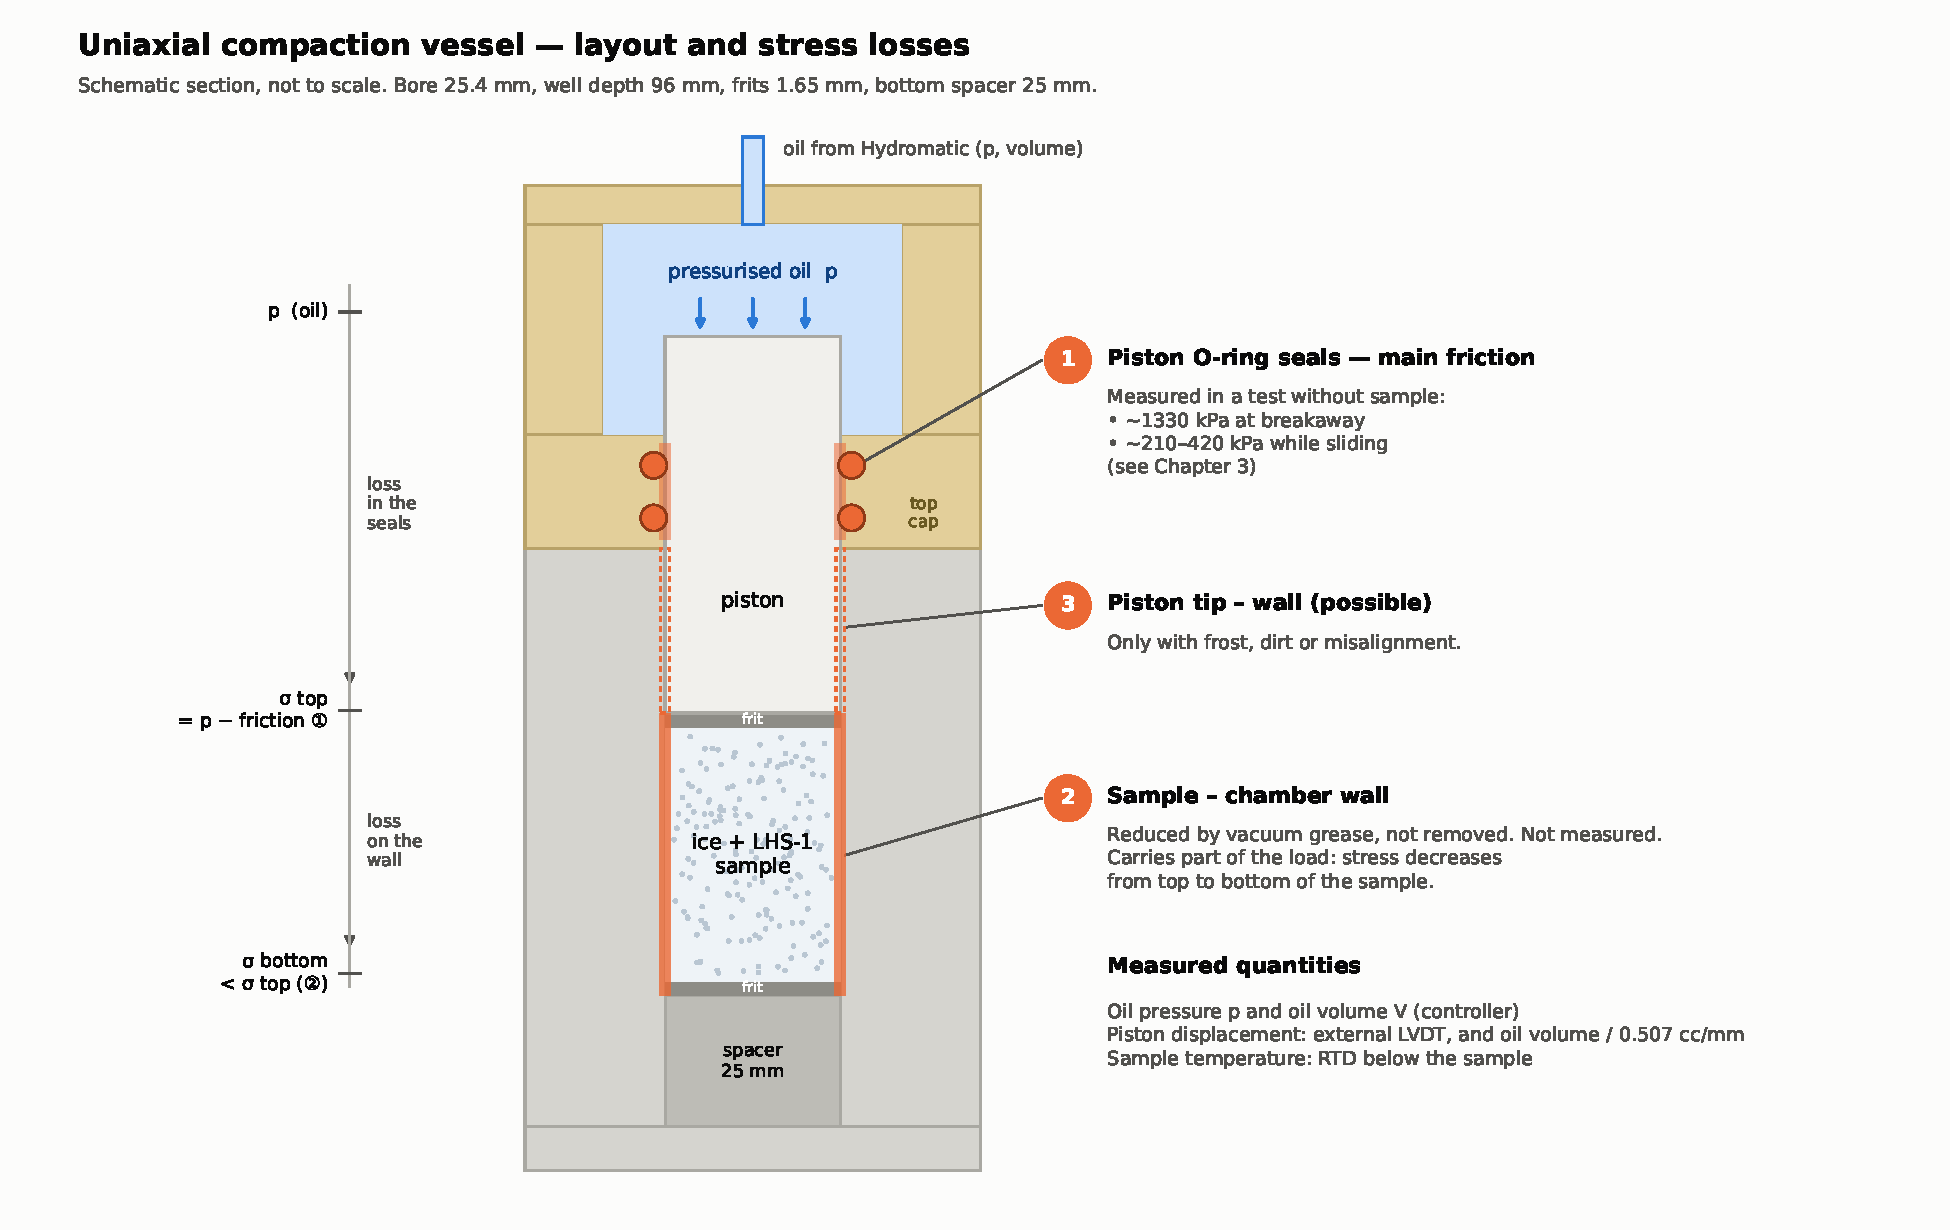
\includegraphics[width=\textwidth]{Images/vessel_schematic.pdf}
    \caption{Schematic cross-section of the uniaxial compaction vessel (not to scale), with the zones where friction reduces the stress transmitted from the oil to the sample. The friction terms are quantified in Chapter~\ref{ch:characterisation}.}
    \label{fig:vessel}
\end{figure}

The vessel can be operated in two ways:
\begin{itemize}
    \item \textbf{pressure control}: the oil pressure is kept constant, so that the axial force on the piston is constant and the sample creeps under a nominally constant stress. This is the mode used in all compaction tests;
    \item \textbf{volume control}: a given volume of oil is pumped into the chamber, which imposes a given piston displacement. This mode was used only to characterise the seal friction (Chapter~\ref{ch:characterisation}).
\end{itemize}

\subsection{Geometry}
\label{subsec:geometry}

\paragraph{Sample chamber.} The sample chamber is a cylindrical bore with a diameter of 25.4\,mm (1\,inch), so that the cross-sectional area of the sample is $A = 5.07$\,cm$^2$. Its depth, measured from the top surface of the vessel to the top of the bottom assembly, is $W = 96$\,mm. The bottom assembly is threaded into the lower end of the vessel and consists of a plug that forms the floor of the chamber, a 25\,mm steel spacer and a threaded closure. It can be removed to extract the sample at the end of the test.
% TODO: confirm the reference surfaces for W = 96 mm with a drawing or a direct measurement.

\paragraph{Porous frits.} The sample is placed between two porous metal frits with a diameter equal to that of the chamber and a thickness $t_f = 1.65$\,mm. The frits distribute the load uniformly over the sample faces and let air escape from the pores during compaction. They are cleaned in an ultrasonic bath, dried and weighed before each test, and cooled in the freezer before being placed in contact with the sample.

\paragraph{Piston.} The piston is a steel cylinder with the same diameter as the chamber, which runs through the top cap of the vessel. It has an axial bore that vents the air expelled from the sample. Its upper end is in the oil chamber and is sealed by O-rings housed in the top cap. Since the oil acts on the full cross-section of the piston, a volume of oil $\Delta V$ pumped into the chamber moves the piston by
\begin{equation}
    \Delta x = \frac{\Delta V}{A} = \frac{\Delta V}{0.507\,\mathrm{cm^3/mm}},
    \label{eq:dx_volume}
\end{equation}
if the oil circuit were perfectly rigid. Equation~\eqref{eq:dx_volume} is the basis of the oil-volume measurement of displacement (Section~\ref{subsec:displacement}); the corrections for the compliance of the circuit are presented in Chapter~\ref{ch:characterisation}.

\paragraph{Sample height.} After the sample is placed in the chamber and the upper frit is placed on it, the depth $d$ from the top surface of the vessel to the top of the upper frit is measured with the depth rod of a caliper. The initial height of the sample is then
\begin{equation}
    H_0 = W - d - 2\,t_f.
    \label{eq:H0}
\end{equation}
At the end of the test, the height of the extracted sample is measured with a caliper, and the length of the piston protruding from the top cap is recorded. The two measurements give independent checks of the final height.

\paragraph{Wall preparation.} Before each test, the chamber, the piston and the threads are cleaned with isopropanol, to remove residual grease and moisture that could freeze on the threads. The chamber wall is then coated with a thin layer of vacuum grease, which reduces the friction between sample and wall and makes extraction easier. Before a new sample is inserted, the piston must be pushed back into its housing, expelling the oil used in the previous test back through the oil line. This is done by striking the piston with a rubber mallet while holding the top cap, with the oil line open.

\subsection{Loading system}
\label{subsec:loading}

\paragraph{Pressure/volume controller.} The oil pressure and volume are controlled by a stand-alone pressure/volume controller (Hydromatic 28-WF45SG, Controls S.p.A.). It consists of a piston pump driven by a stepper motor along a linear track, with a volume capacity of 250\,cm$^3$, and controlled by a touch-screen panel. Its main specifications are~\cite{hydromatic2018}:
\begin{itemize}
    \item maximum pressure 3500\,kPa;
    \item pressure resolution 0.1\,kPa;
    \item volume resolution 0.001\,cm$^3$, equivalent through Equation~\eqref{eq:dx_volume} to a piston displacement of 2\,$\mu$m;
    \item operating temperature of the controller +15 to +40\,$^\circ$C, so that the controller sits in the laboratory, outside the freezer.
\end{itemize}

The controller runs a programmed sequence of up to 15 steps. Each step consists of a ramp to a target value of pressure or volume, with a prescribed duration, followed by a hold at the target for a prescribed time. For each ramp and hold, the user selects whether the change in volume is measured and whether the volume reading is reset to zero at the start of the step. The internal data logging can be linear in time, or follow a power law or a geometric progression, so that more readings are taken at the start of a step. Upper and lower pressure limits can be set; when a limit is exceeded, the controller can sound an alarm, hold or stop the test. The upper limit must be set sufficiently above the target pressure, otherwise the overshoot at the end of a fast ramp stops the test (Chapter~\ref{ch:characterisation}).

\paragraph{Oil circuit.} The controller is connected to the vessel by a line that runs from the laboratory into the freezer. The circuit has two valves:
\begin{itemize}
    \item a valve at the wall, which connects the line to the oil reservoir. It is opened when the piston is pushed back between tests, so that the expelled oil can return to the reservoir, and closed during tests;
    \item an L-shaped valve inside the freezer, between the line and the vessel. When it is closed, the controller can pressurise the line up to the vessel without loading the sample; opening it applies the pressure to the piston.
\end{itemize}
The second valve allows the sample to be loaded with a step of stress: the line is first brought to the target pressure with the valve closed, and the valve is then opened. This is the loading procedure used in the firn compaction experiments and adopted in this thesis (Chapter~\ref{ch:characterisation}).

\paragraph{Range of axial stress.} The maximum oil pressure of 3.5\,MPa is also, to a first approximation, the maximum axial stress on the sample, since the oil acts on a piston of the same diameter as the sample. The stress actually transmitted to the sample is lower, because part of the force is taken by the friction of the piston seals and by the friction between sample and wall (Figure~\ref{fig:vessel}). In this thesis the target pressures range from 0.5 to 3.4\,MPa.

\subsection{Displacement measurement}
\label{subsec:displacement}

\paragraph{LVDT.} The displacement of the piston is measured outside the vessel by a linear variable differential transformer (LVDT), mounted on the top cap and touching a flat plate fixed to the piston. The LVDT has a resolution of about 1\,$\mu$m~\cite{skarbek2025data}. Its calibration is valid only for negative readings, that is, with the core pushed in beyond its zero position: the LVDT must be set at the start of each test so that the reading is negative, and the readings close to zero are unreliable. In the configuration used, the reading saturates at about $-19.6$\,mm.
% TODO: LVDT model, nominal stroke and calibration factor.
The usable stroke of the LVDT is therefore smaller than the total compaction of a loose sample, which can exceed 20\,mm. How the LVDT is set to cover the time-dependent stage of the test is described in Chapter~\ref{ch:characterisation}.

\paragraph{Oil volume.} The volume of oil delivered by the controller provides a second, independent measurement of the piston displacement through Equation~\eqref{eq:dx_volume}. It covers the whole stroke of the piston, including the fast compaction at the start of the test, which the LVDT cannot follow when it goes out of range. The oil volume is affected by the compressibility of the oil, the expansion of the line under pressure, possible leaks and temperature changes of the oil in the line. These effects are measured and corrected as described in Chapter~\ref{ch:characterisation}.

\subsection{Temperature control}
\label{subsec:temperature}

The sample chamber is surrounded by an outer jacket through which chilled methanol is circulated by a refrigerated circulator (Julabo Magio MS-1000F). The temperature is measured by a resistance temperature detector (RTD) placed close to the bottom surface of the sample, which is also the control sensor of the circulator. The whole vessel is housed in a chest freezer, which provides additional insulation and reduces the temperature gradient along the vessel. With this setup the sample temperature can be controlled down to $-40\,^\circ$C with a precision of 0.05\,$^\circ$C~\cite{skarbek2025data}.

Before loading, the sample is left in the closed vessel for at least one hour to reach a uniform temperature. Only the vessel is temperature-controlled: the controller and most of the oil line are at laboratory temperature, which changes between day and night. The effect of these changes on the oil volume is discussed in Chapter~\ref{ch:characterisation}.

\subsection{Data acquisition}
\label{subsec:daq}

The data are recorded by a data logger (Geodatalog 8, Controls S.p.A.) controlled by the DATACOMM~2 software on a laboratory computer, through a dedicated Ethernet connection~\cite{geodatalog2020}. The logger has eight independent input channels with an effective resolution of 131\,000 points and can sample up to 500 readings per second per channel. Three quantities are recorded:
\begin{itemize}
    \item the LVDT displacement, from an analogue input channel of the logger;
    \item the oil pressure and the oil volume, read from the pressure/volume controller through the network, so that all three are recorded with the same time base.
\end{itemize}
All tests were logged at 1\,Hz, the same rate as the firn compaction experiments. This rate resolves the fast compaction in the first seconds after loading and gives files of manageable size (about 225\,000 rows for a test of 62\,h). The controller also stores its own record of pressure and volume, which is used as a backup.
% TODO: check that the computer is not connected to the external network during tests (lab rule), and mention it if relevant.

The sample temperature is recorded by the circulator.
% TODO: check whether the RTD temperature is logged with the other channels or only displayed by the circulator; if logged, give the channel and rate.


\chapter{Apparatus characterisation and test procedure}
\label{ch:characterisation}%
% Aim: 15-20 pages. This is an original contribution of the thesis: how the measured oil pressure and
% displacement are turned into stress and strain on the sample, and with what uncertainty.

The compaction vessel measures three quantities: the oil pressure $p$, the volume of oil $V$ delivered by the controller and the reading $x$ of the external LVDT. What is needed are the axial stress on the sample and its height as functions of time. Between the two there are several sources of error: the friction of the piston seals, the compliance of the oil circuit, the limited range of the LVDT, leaks, temperature changes of the oil in the line and the friction between the sample and the chamber wall. This chapter quantifies each of them, using a test without a sample and the first compaction tests, and derives the test procedure, the data reduction and the uncertainty budget used in the rest of the thesis.

The tests used for the characterisation are listed in Table~\ref{tab:commissioning}. They were carried out in the first weeks of the campaign, while the procedure was being developed. Their compaction results are reported in Appendix~\ref{app:tests}; here they serve only to characterise the apparatus.

\begin{table}[H]
    \centering
    \caption{Tests used to characterise the apparatus.}
    \label{tab:commissioning}
    \begin{tabularx}{\textwidth}{|l|>{\raggedright\arraybackslash}p{4.2cm}|>{\raggedright\arraybackslash}X|}
        \hline
        \textbf{Test} & \textbf{Sample and conditions} & \textbf{Used for} \\
        \hline
        F199 & no sample; volume control, 4.9\,cm$^3$ in 10\,min & seal friction; LVDT against oil volume \\
        \hline
        F202 & first loading trials & behaviour of the controller in volume control and with pressure limits \\
        \hline
        F203 & 18\,g of granular ice, $-10\,^\circ$C, target 3\,MPa, 1.5\,h & compliance on unloading; oil-volume displacement checked against measured heights \\
        \hline
        F204 & 12.25\,g ice + 12.25\,g quartz sand, $-20\,^\circ$C, 2\,MPa, 41\,h with unload--reload & seal friction during the step load; LVDT range; compliance; leak; thermal drift \\
        \hline
    \end{tabularx}
\end{table}

% ---------------------------------------------------------------------------
\section{Piston seal friction}
\label{sec:seal_friction}
% ---------------------------------------------------------------------------

\subsection{Measurement without a sample}

The O-rings that seal the oil chamber around the piston (Figure~\ref{fig:vessel}) resist the motion of the piston. With no sample in the chamber, the piston moves as soon as the oil pressure overcomes this friction, and the oil pressure recorded while the piston moves is a direct measurement of the seal friction expressed as a stress, $\sigma_{\mathrm{seal}}$. The same approach was used to calibrate the seal friction of the vessel for the firn compaction experiments~\cite{firn_inprep}.

In test F199 the piston, previously pushed back into its housing, was driven into the empty chamber in volume control, by pumping 4.9\,cm$^3$ of oil in about 10 minutes. The piston moved by 9.25\,mm at an average velocity of about 15\,$\mu$m/s. Figure~\ref{fig:seal_friction} shows the oil pressure as a function of the piston displacement measured by the LVDT. Three features are evident:
\begin{itemize}
    \item \textbf{a breakaway peak} of 1330\,kPa at the very start (0.23\,mm of displacement): this is the static friction of seals that have been at rest, after the piston was struck back into place;
    \item \textbf{a transition} over the first 1.7\,mm, during which the pressure falls from about 1000\,kPa to the sliding level;
    \item \textbf{a sliding level} with a mean of 420\,kPa, varying between 340 and 570\,kPa with the position of the piston, with a broad local maximum at about 5.4\,mm.
\end{itemize}

\begin{figure}[H]
    \centering
    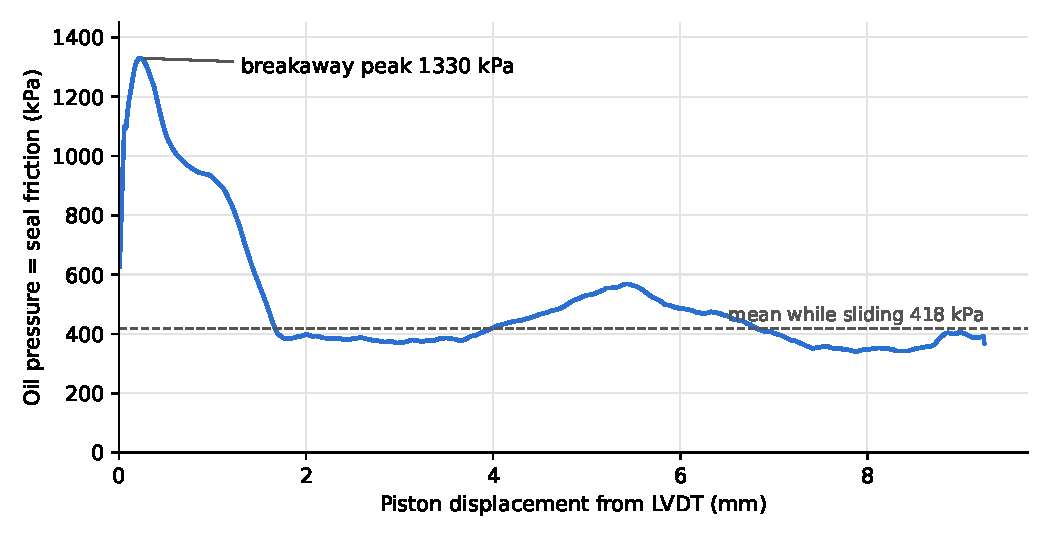
\includegraphics[width=0.85\textwidth]{Images/fig_seal_friction.pdf}
    \caption{Oil pressure against piston displacement in the test without a sample (F199, volume control, about 15\,$\mu$m/s). The pressure equals the seal friction.}
    \label{fig:seal_friction}
\end{figure}

\subsection{Measurement during a test}

The seal friction can also be read during the step load of each compaction test. When the valve to the vessel is opened, the line, pressurised to the target, discharges into the oil chamber and the piston moves quickly towards the sample, through the gap above the upper frit and into the loose sample. While the piston runs with little resistance from the sample, the pressure drops to the level needed to overcome the seals, and stays there until the sample starts to resist. In F204 (Figure~\ref{fig:start}a) this level was $215\pm8$\,kPa between 2 and 7\,s after opening, at a piston velocity of about 1.8\,mm/s. In F203 it was about 220\,kPa.

The in-test value is lower than the sliding level measured in F199. Two effects contribute. The piston is at a different position in its housing in each test, and F199 showed that the friction changes with position. The velocity differs by two orders of magnitude, and elastomer seals generally show lower friction at higher sliding velocities. Moreover, the pressure is measured at the controller, so during fast flow it slightly overestimates the pressure in the oil chamber, which would make the true in-test friction even lower.

\subsection{Consequences for the applied stress}

The axial stress applied by the piston to the top of the sample is
\begin{equation}
    \sigma_a = p - \sigma_{\mathrm{seal}},
    \label{eq:sigma_a}
\end{equation}
where $\sigma_{\mathrm{seal}}$ is the friction that acts against the motion of the piston. During a compaction test the piston never stops, since the sample keeps creeping, so the relevant value is the sliding friction at the very low velocities of the creep stage (about 1\,$\mu$m/s after 15\,min and 0.1\,$\mu$m/s after 2\,h in F204). It has not been measured directly at these velocities.
% TODO: run the empty-vessel test at 2-3 flow rates spanning 0.1-100 um/s and over the full stroke used in the tests, as in the firn calibration.
In the firn compaction experiments, empty-vessel tests at velocities from about 0.1 to 100\,$\mu$m/s gave a seal friction that depended on the piston displacement but little on velocity, except at the slowest velocity for displacements above about 12\,mm~\cite{firn_inprep}.

In this thesis $\sigma_{\mathrm{seal}}$ is taken, for each test, as the plateau of pressure measured during the step load, and the range 210--420\,kPa found above is used to estimate its uncertainty (Section~\ref{sec:uncertainty}). Two consequences follow.
\begin{itemize}
    \item \textbf{Minimum target pressure.} An uncertainty of about $\pm100$\,kPa on $\sigma_{\mathrm{seal}}$ is $\pm5\%$ of the applied stress at a target of 2\,MPa, but $\pm25\%$ at 0.5\,MPa. Targets below about 1\,MPa are therefore affected by a large uncertainty, unless the seal friction is calibrated as a function of position and velocity.
    \item \textbf{Static friction on reloading.} When the piston has been at rest, it can only move again once the oil pressure exceeds the static friction, which may be close to the breakaway value of 1330\,kPa. While the piston is stationary, the stress on the sample is not known: it lies anywhere between $p - \sigma_{\mathrm{static}}$ and $p$. This matters for the interpretation of unloading--reloading stages: if the piston does not move on reloading, this may be due to the sample being stiffer, to the static friction of the seals, or both (Chapter~\ref{ch:results}).
\end{itemize}

% ---------------------------------------------------------------------------
\section{System compliance}
\label{sec:compliance}
% ---------------------------------------------------------------------------

When the pressure rises, part of the oil delivered by the controller does not move the piston: it is stored in the circuit by the compressibility of the oil and by the expansion of the tubing, fittings and chambers. The volume stored as a function of pressure, $S(p)$, must be subtracted before the oil volume is converted into displacement.

$S(p)$ was measured during the final unloading of each test. At that stage the sample has been compacted for hours under the target stress, and the piston does not move appreciably while the pressure is decreased from the target to about 10\,kPa: the volume of oil returned to the controller is the volume released by the circuit. Figure~\ref{fig:compliance} shows the curves measured in F203 and F204. They are slightly non-linear, stiffer at higher pressures:
\begin{itemize}
    \item about 0.62\,cm$^3$/MPa between 0 and 0.5\,MPa;
    \item about 0.49\,cm$^3$/MPa between 0.5 and 1\,MPa;
    \item about 0.43\,cm$^3$/MPa between 1 and 2\,MPa.
\end{itemize}
In total, about 1.0\,cm$^3$ of oil is stored at 2\,MPa and 1.45\,cm$^3$ at 3\,MPa. Through Equation~\eqref{eq:dx_volume}, 1\,cm$^3$ corresponds to 2\,mm of apparent piston travel, so the compliance correction is of the same order as the creep compaction and cannot be neglected. The two curves differ by about 5\% at 2\,MPa, a difference that can come from the different volume of oil in the chamber (different piston position) and from small amounts of trapped air.

\begin{figure}[H]
    \centering
    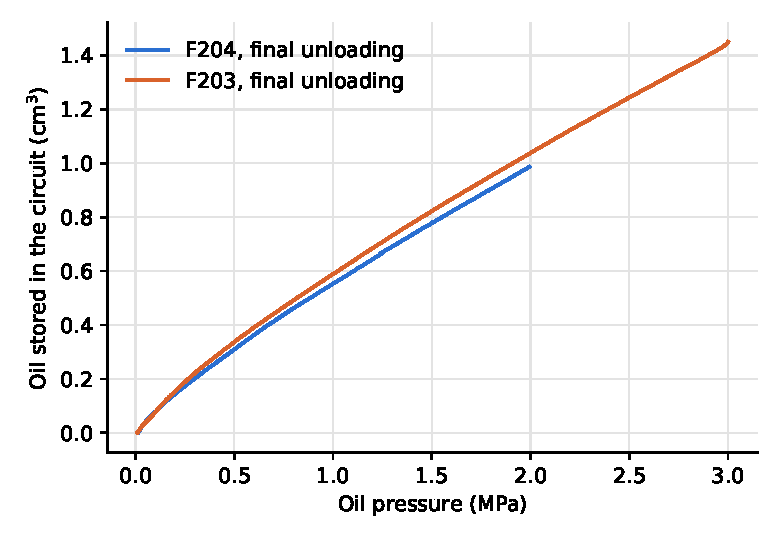
\includegraphics[width=0.62\textwidth]{Images/fig_compliance.pdf}
    \caption{Volume of oil stored in the circuit as a function of the oil pressure, measured during the final unloading of tests F203 and F204, with the piston stationary.}
    \label{fig:compliance}
\end{figure}

The unloading method assumes that the sample does not expand during unloading. Any elastic rebound of the sample pushes the piston up and returns additional oil, so the measured $S(p)$ is an upper bound of the circuit compliance. A direct measurement, independent of the sample, can be obtained by pressurising the line against the closed valve before each test, which is already part of the loading procedure (Section~\ref{sec:procedure}). This measures the compliance of the line and controller, but not that of the oil chamber in the vessel.
% TODO: record volume and pressure during the closed-valve pressurisation in every test, and compare with the unloading curve.

% ---------------------------------------------------------------------------
\section{Displacement measurement and its limits}
\label{sec:lvdt}
% ---------------------------------------------------------------------------

\subsection{Agreement between LVDT and oil volume}

In the test without a sample (F199) the pressure stayed below 600\,kPa during most of the motion, so the compliance correction was small. A linear fit of the oil volume against the LVDT displacement gave 0.505\,cm$^3$/mm, against the value of 0.507\,cm$^3$/mm expected from the piston area. The two measurements agree within 0.5\%.

At the start of F204 (Figure~\ref{fig:start}b), during the fast run of the piston into the sample, the displacement computed from the oil volume (with the compliance correction) matched the LVDT within 0.05\,mm between 3 and 10\,mm of travel. This confirms that the oil volume gives a reliable measurement of the piston displacement, including during fast events.

\begin{figure}[H]
    \centering
    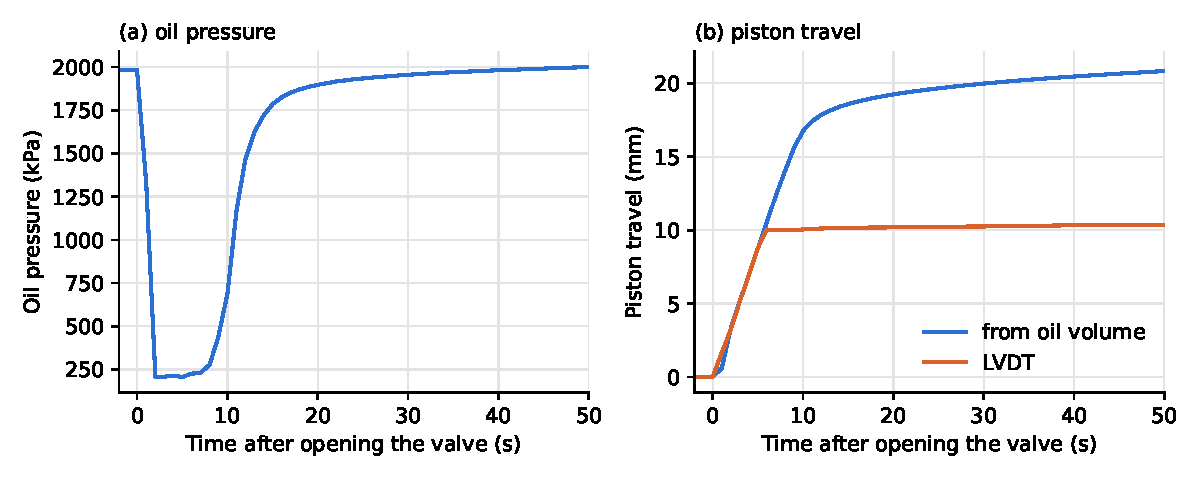
\includegraphics[width=\textwidth]{Images/fig_start.pdf}
    \caption{First 50\,s of test F204 after the valve to the vessel was opened: (a) oil pressure; (b) piston travel from the oil volume (corrected for compliance) and from the LVDT. The LVDT reached the end of its range after 10\,mm of travel.}
    \label{fig:start}
\end{figure}

\subsection{Range of the LVDT}

The LVDT is calibrated for negative readings only, and the readings close to zero are unreliable. At the other end, its reading stopped following the piston at about $-19.6$\,mm in F204, after 10\,mm of travel from the starting position of $-9.55$\,mm (Figure~\ref{fig:start}b). In F203 the reading also stayed almost constant, at about $-17.7$ to $-18.3$\,mm, while the oil volume and the measured final height showed several millimetres of further compaction. The usable interval of the LVDT is therefore from about $-6$ to about $-17$\,mm, that is, about 11\,mm.
% TODO: check the LVDT range with a caliper or gauge blocks over the whole stroke and give the calibrated interval.

The total compaction of a loose sample (about 20\,mm in F203 and F204) exceeds this interval, and most of it takes place in the first minute of the test. With the procedure used in these tests, in which the LVDT is set before loading, the LVDT runs out of range during the step load and cannot measure the creep stage, which is the part of the test where its resolution is most needed. Two remedies are possible:
\begin{enumerate}
    \item reset the LVDT after the step load: once the fast compaction is over (a few minutes after loading), the LVDT body is moved so that the reading returns to about $-6$\,mm, and the offset is recorded. The creep stage, with a compaction of a few millimetres, then falls within the usable interval;
    \item replace the LVDT with one of longer stroke (at least 30\,mm).
\end{enumerate}
In both cases, the oil volume remains the reference for the step load, and the two measurements overlap during the creep stage, which allows the oil-volume corrections to be checked.

% ---------------------------------------------------------------------------
\section{Leakage and thermal drift}
\label{sec:drift}
% ---------------------------------------------------------------------------

During a long test, the oil volume can change for two reasons unrelated to the motion of the piston: oil leaking out of the circuit, and thermal expansion or contraction of the oil in the part of the line that is at laboratory temperature. Both were observed in F204, in the stages after the main creep stage (Figure~\ref{fig:drift_leak}).

\begin{figure}[H]
    \centering
    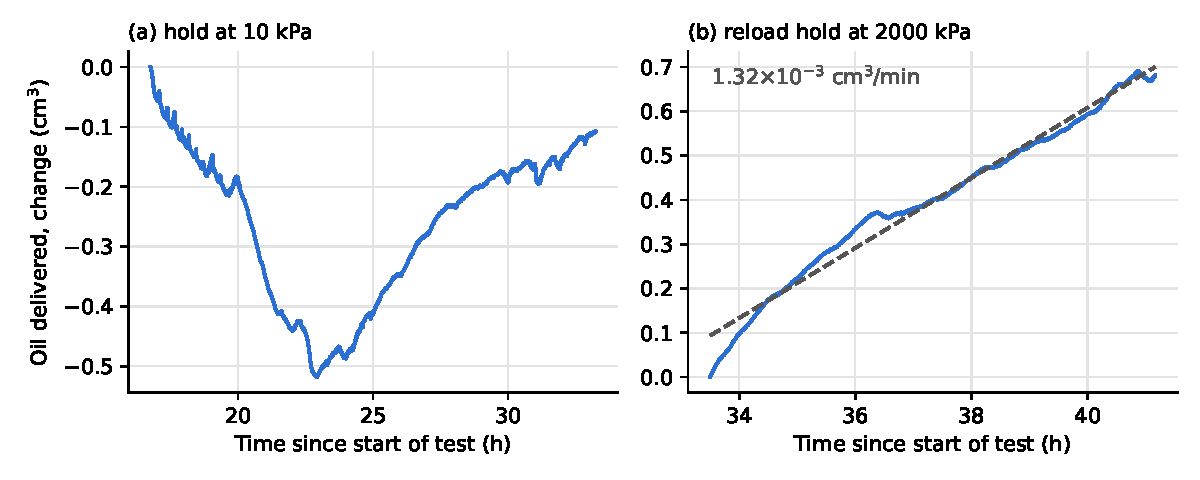
\includegraphics[width=\textwidth]{Images/fig_drift_leak.pdf}
    \caption{Oil volume during (a) the 16.6\,h hold at 10\,kPa and (b) the 7.6\,h reload hold at 2000\,kPa of test F204. In (b) the dashed line is a linear fit.}
    \label{fig:drift_leak}
\end{figure}

\paragraph{Thermal drift.} During the hold at 10\,kPa (Figure~\ref{fig:drift_leak}a), when the oil pressure is too low to cause a leak or to move the piston, the oil volume changed by about 0.5\,cm$^3$ over a day, decreasing and then increasing again with a minimum in the early afternoon. The controller keeps the pressure constant, so when the oil in the line warms up and expands, oil is withdrawn into the controller, and the opposite happens when it cools down. A day--night oscillation of $\pm0.25$\,cm$^3$ corresponds to an apparent displacement of $\pm0.5$\,mm. Part of the change in the first hours of this stage may also be due to elastic rebound of the sample after unloading; the two effects cannot be separated with the data of F204.

\paragraph{Leak.} During the reload hold at 2000\,kPa (Figure~\ref{fig:drift_leak}b) the controller delivered oil at a nearly constant rate of $1.32\times10^{-3}$\,cm$^3$/min. A constant rate over 7.6\,h is not what is expected from creep of the sample, which decelerates in time (log-linear compaction, Section~\ref{sec:firn}). It is therefore attributed to a leak, either through the piston seals or at a fitting of the line. Over the 16.6\,h of the main creep stage of F204, a leak of this size amounts to 1.3\,cm$^3$, or 2.6\,mm of apparent travel, which is about a third of the measured creep compaction. In the data reduction the leak is subtracted at a constant rate (Section~\ref{sec:data_reduction}).

Whether the leak is in the line or in the vessel can be established with a simple test: the line is pressurised to 2\,MPa against the closed valve for 2--3\,h. If the volume stays constant, the leak is in the vessel (seals); if oil is still delivered, it is in the line or the controller.
% TODO: run the leak test, find and fix the leak; report the result here.
A leak test of this kind, and a hold of a rigid dummy sample (a steel cylinder) at constant pressure, should be carried out periodically, so that the drift correction is based on a direct measurement rather than on the late stages of a compaction test.

% ---------------------------------------------------------------------------
\section{Sample--wall friction}
\label{sec:wall_friction}
% ---------------------------------------------------------------------------

As the sample is compressed, the radial stress against the chamber wall mobilises a shear stress along the wall that opposes the downward motion of the sample. Part of the axial force applied at the top is therefore carried by the wall, and the axial stress decreases with depth. This effect is well known in powder compaction and in oedometer testing. For a uniform coefficient of wall friction $\mu$ and a constant ratio $K$ between radial and axial stress, equilibrium of a slice of sample gives the classical exponential decay
\begin{equation}
    \sigma_z(z) = \sigma_a\,\exp\left(-\frac{4\,\mu K\,z}{D}\right),
    \label{eq:janssen}
\end{equation}
where $z$ is the depth below the top of the sample and $D$ its diameter. The mean axial stress over a sample of height $H$ is then
\begin{equation}
    \bar\sigma_z = \sigma_a\,\frac{1-\exp(-\beta)}{\beta}, \qquad \beta = \frac{4\,\mu K\,H}{D}.
    \label{eq:janssen_mean}
\end{equation}

The wall of the chamber is coated with a thin film of vacuum grease (Section~\ref{subsec:geometry}), which reduces $\mu$ but does not eliminate it, especially at low temperature, where the grease becomes stiffer. Neither $\mu$ nor $K$ was measured in this work: the vessel has no load cell at the bottom of the sample, so the force transmitted to the base cannot be compared with that applied at the top.

An order of magnitude can be obtained with plausible values. For granular materials in oedometric compression $K = K_0\approx0.4$--0.5, and for ice-rich materials, which behave more like a viscous fluid, $K$ approaches 1. With $\mu = 0.05$--0.10 for a greased steel wall and the height-to-diameter ratios of the tests ($H/D = 1.5$--2.4):
\begin{itemize}
    \item for $\mu K = 0.025$ (low friction), $\beta\approx0.15$--0.24, and the mean stress is 7--11\% lower than $\sigma_a$;
    \item for $\mu K = 0.10$ (high friction), $\beta\approx0.6$--1.0, and the mean stress is 25--37\% lower than $\sigma_a$.
\end{itemize}
The effect is therefore potentially larger than that of the seal friction, it acts in one direction only (it always reduces the stress), and it decreases as the sample becomes shorter during compaction. It also makes the stress non-uniform along the sample, so that the upper part densifies faster than the lower part.

Three measures limit this source of error. First, the wall is greased before every test. Second, the samples should be as short as practical: the firn experiments on the same vessel used samples about 45\,mm high ($H/D\approx1.8$), and for the mixtures of this thesis a height of 30--40\,mm ($H/D\approx1.2$--1.6) would halve $\beta$ with respect to the first tests. Third, the stresses are reported as $\sigma_a$ (the stress at the top of the sample), with the wall friction treated as a systematic error in the uncertainty budget.
% TODO: if possible, measure the density profile of a compacted sample (slices) to quantify the stress gradient.

% ---------------------------------------------------------------------------
\section{Test procedure}
\label{sec:procedure}
% ---------------------------------------------------------------------------

The procedure adopted is that of the firn compaction experiments on the same vessel, modified where the characterisation above showed it necessary. The step-by-step protocol is given in Appendix~\ref{app:protocol}; its main stages are the following.

\begin{enumerate}
    \item \textbf{Preparation of the vessel.} The chamber, piston and threads are cleaned with isopropanol; the wall is greased; the piston is pushed back into its housing with the reservoir valve open; the frits are cleaned, weighed and cooled (Section~\ref{subsec:geometry}).
    \item \textbf{Sample placement.} The sample is prepared in the cold room (Section~\ref{subsec:mixtures}) and placed in the chamber between the frits. The depth of the upper frit is measured to obtain $H_0$ (Equation~\eqref{eq:H0}), and the top cap is screwed on.
    \item \textbf{Thermal equilibration.} The sample is left in the closed vessel at the test temperature for at least one hour.
    \item \textbf{Setting the instruments.} The LVDT is set at a negative reading and its initial value recorded. The controller is programmed with the step table and with an upper pressure limit at least 400\,kPa above the target, so that the overshoot at the end of the step does not stop the test. The reservoir valve is closed, and data logging is started at 1\,Hz.
    \item \textbf{Pressurisation against the closed valve.} With the valve to the vessel closed, the controller brings the line to the target pressure. The LVDT must not move: this checks that the valve is closed and the line holds pressure.
    \item \textbf{Step load.} The valve to the vessel is opened. The piston runs into the sample, the pressure drops to the seal-friction level and then recovers to the target as the sample takes the load (Figure~\ref{fig:start}). The time of opening is recorded.
    \item \textbf{Creep stage.} The pressure is held constant for the planned duration. If the LVDT has gone out of range, it is reset to about $-6$\,mm a few minutes after loading, and the offset is recorded (Section~\ref{sec:lvdt}).
    \item \textbf{Unloading.} The pressure is reduced to about 10\,kPa with a slow ramp (30--45\,min), which gives the compliance curve $S(p)$ (Section~\ref{sec:compliance}).
    \item \textbf{End of test.} The piston protrusion is measured, the bottom of the vessel is removed and the sample is extracted. Its height and mass, and the mass of the frits, are measured immediately.
\end{enumerate}

The step load with the closed valve reproduces the procedure used for firn and makes the tests comparable with those data. Its drawback, for loose samples, is that the piston runs at high speed through the gap and into the sample, so that the first part of the compaction occurs at an unknown and varying stress. An alternative is to bring the piston into contact with the sample at a small seating stress (about 50\,kPa) before the step load, by advancing it slowly in volume control. This eliminates the gap and defines the initial state of the sample under a known stress.

\subsection{Detection of contact}

In F204 the pressure stayed at the seal-friction level for about 7\,s after the valve was opened (Figure~\ref{fig:start}a). During this time the piston travelled about 12\,mm, while the gap between piston and sample, obtained from the geometry, was only 5.8\,mm. The pressure therefore does not identify the moment of geometric contact: a loose sample is compressed by several millimetres while offering a resistance below the resolution of the pressure measurement (a few tens of kilopascals above the seal friction). The rise of the pressure above the sliding level identifies instead the moment at which the sample starts to carry a significant stress.

For this reason, the contact is defined geometrically: the gap $g$ between the lower face of the piston and the upper frit before the test is obtained from the piston length and the depth of the upper frit. The initial height $H_0$ is assigned to the sample at the moment when the piston travel equals $g$. If $g$ is not measured, it can be obtained a posteriori from the total piston travel and the measured final height (Section~\ref{sec:data_reduction}).

% ---------------------------------------------------------------------------
\section{Data reduction}
\label{sec:data_reduction}
% ---------------------------------------------------------------------------

The raw data of each test are the time series $p(t)$, $V(t)$ and $x(t)$ at 1\,Hz. They are reduced as follows.

\paragraph{Piston travel.} The piston travel since the opening of the valve, $u(t)$, is computed from the oil volume:
\begin{equation}
    u(t) = \frac{\Delta V(t) - \left[S(p(t)) - S(p_0)\right] - q\,(t-t_0)}{A},
    \label{eq:travel}
\end{equation}
where $\Delta V(t)$ is the volume delivered since the valve was opened at time $t_0$ (including the volume released by the pressurised line), $S(p)$ is the compliance curve measured at unloading, $p_0$ is the pressure just before opening, $q$ is the leak rate and $A = 0.507$\,cm$^3$/mm. Where the LVDT is within its usable range, its readings are used to check $u(t)$.

\paragraph{Sample height.} The height of the sample is
\begin{equation}
    H(t) = H_0 - \lambda\left[u(t) - g\right], \qquad u\ge g,
    \label{eq:height}
\end{equation}
where $\lambda$ is a scale factor that makes the computed final height equal to the measured one, $H_f$. For an ideal set of corrections $\lambda = 1$. In F203 the factor was 1.009, and in F204, with the leak correction, 0.94. The difference from unity measures the residual error of the corrections and is reported for every test.

\paragraph{Void ratio, density and porosity.} With the height of solids $H_s$ (Equation~\eqref{eq:e0}) and the total mass $M = m_i + m_s$:
\begin{equation}
    e(t) = \frac{H(t)}{H_s} - 1, \qquad
    \rho(t) = \frac{M}{A\,H(t)}, \qquad
    n(t) = \frac{e(t)}{1+e(t)}.
    \label{eq:state}
\end{equation}
The mass $M$ is taken from the weighed components and checked against the mass of the sample after the test. For pure ice, the relative density $D = \rho/\rho_i$ is also used, to compare with the firn literature.

\paragraph{Axial stress.} The applied axial stress is computed with Equation~\eqref{eq:sigma_a}, using the seal friction measured during the step load of the same test.

\paragraph{Time origin.} Following the firn experiments, the origin of the compaction time is set at the moment when the oil pressure first reaches 99\% of the target after the valve is opened. In F204 this occurred 40\,s after opening. The compaction before this moment is the loading stage, reported separately.

\paragraph{Strain rate.} The axial strain rate is
\begin{equation}
    \dot\varepsilon = -\frac{1}{H}\frac{\mathrm{d}H}{\mathrm{d}t}.
    \label{eq:strain_rate}
\end{equation}
Differentiating data recorded at 1\,Hz amplifies the noise. Following the firn experiments, $H(t)$ is fitted with a straight line in $\log_{10} t$ over a moving window of constant width in log-time, $[\log_{10}t - 0.1,\ \log_{10}t + 0.1]$. The derivative of the fit at the centre of the window gives $\mathrm{d}H/\mathrm{d}t$. The window therefore covers a few seconds at the start of the creep stage and several hours at its end.

\paragraph{Coefficient of secondary compression.} Where the void ratio decreases linearly with the logarithm of time, the slope gives the coefficient of secondary compression (Equation~\eqref{eq:isotache}):
\begin{equation}
    C_\alpha = -\frac{\Delta e}{\Delta\log_{10}t},
    \label{eq:calpha}
\end{equation}
fitted between 1 and 100\,min of compaction time unless stated otherwise.

% ---------------------------------------------------------------------------
\section{Uncertainty budget}
\label{sec:uncertainty}
% ---------------------------------------------------------------------------

Table~\ref{tab:uncertainty} summarises the sources of error discussed in this chapter and their effect on the main quantities, for a typical test at a target of 2\,MPa with a sample of about 60\,mm initial height.

\begin{table}[H]
    \centering
    \caption{Uncertainty budget for a typical test (target 2\,MPa, $H_0\approx60$\,mm, 16\,h of creep). Systematic errors act in one direction; random errors are given as $\pm$.}
    \label{tab:uncertainty}
    \footnotesize
    \renewcommand{\arraystretch}{1.15}
    \begin{tabularx}{\textwidth}{|>{\raggedright\arraybackslash}p{3.1cm}|>{\raggedright\arraybackslash}p{3.3cm}|>{\raggedright\arraybackslash}X|}
        \hline
        \textbf{Source} & \textbf{Size} & \textbf{Effect} \\
        \hline
        Seal friction & 210--420\,kPa & $\sigma_a$: $\pm5\%$ at 2\,MPa, $\pm25\%$ at 0.5\,MPa \\
        \hline
        Wall friction & $\mu K$ = 0.025--0.10 & mean stress 7--37\% below $\sigma_a$ (systematic) \\
        \hline
        Compliance $S(p)$ & $\pm5\%$ of 1.0\,cm$^3$ & travel $\pm0.1$\,mm; $e$: $\pm0.003$ \\
        \hline
        Leak & $\pm30\%$ of $1.3\times10^{-3}$\,cm$^3$/min & travel $\pm0.8$\,mm after 16\,h; $e$: $\pm0.02$; $C_\alpha$ at late times \\
        \hline
        Thermal drift & $\pm0.25$\,cm$^3$ (day--night) & travel $\pm0.5$\,mm; $e$: $\pm0.015$; spurious oscillations in $\dot\varepsilon$ \\
        \hline
        Initial height & $\pm0.1$\,mm & $e$: $\pm0.003$ \\
        \hline
        Grain density of LHS-1 & 2.75--2.81\,g/cm$^3$ & $H_s$: up to 1\% (equal volumes of ice and simulant); $e$: $\pm0.01$ \\
        \hline
        Mass loss & 0.5\,g of ice & $e_f$: +0.03 (systematic, checked by final weighing) \\
        \hline
        Temperature & $\pm0.05\,^\circ$C & creep rate $\pm0.6\%$ (with $Q = 60$\,kJ/mol) \\
        \hline
    \end{tabularx}
\end{table}

The uncertainties on the void ratio are absolute. They matter most at the end of the test, when the void ratio is small: an error of $\pm0.03$ is 6\% of the void ratio at $e = 0.5$ but 60\% at $e = 0.05$. The uncertainties on displacement are reduced by anchoring the computed height to the measured initial and final heights (Equation~\eqref{eq:height}): the anchoring removes the cumulative error at the end of the test, but not the error in the shape of the curve between the two ends.

The main conclusions are three. First, the stress is known to about $\pm5\%$ from the seal friction at targets of 2\,MPa and above, but the wall friction may reduce the mean stress in the sample by a larger and unknown amount; this is the largest source of uncertainty in the comparison between tests at different stresses and between the vessel and other apparatus. Second, the leak and the thermal drift control the uncertainty of the late creep stage, after about 100\,min, and must be measured and, if possible, eliminated. Third, temperature control is not a significant source of error. The improvements identified in this chapter (shorter samples, LVDT reset after loading, leak test, seal friction calibration over the stroke) are summarised in Chapter~\ref{ch:conclusions}.


\chapter{Experimental results}
\label{ch:results}%
% Aim: 20-25 pages. Present observations first; interpretation comes at the end of the chapter and in Chapter 5.

\section{Experimental programme}
\label{sec:programme}
% Table of all tests: ID, ice content, temperature, target pressure, corrected stress,
% initial height and density, duration, remarks. State which tests are excluded and why.

\section{Pure ice}
\label{sec:results_ice}
% Validation of procedure and data reduction against the published pure-ice compaction data from the same vessel.
\subsection{Compaction during loading}
\subsection{Compaction under constant stress}
% Height versus log-time; densities at fixed times; strain rate versus density.

\section{Ice--regolith mixtures}
\label{sec:results_mixtures}
\subsection{Effect of temperature}
\subsection{Effect of ice content}
\subsection{Effect of axial stress}

\section{Dry regolith}
\label{sec:results_dry}
% Reference test for the skeleton-only end-member; comparison with literature oedometric data.

\section{Unloading and reloading}
\label{sec:results_unloading}
% Dead band due to seal friction; unloading modulus from the slope where the piston moves.

\section{Constant-rate compression and stress relaxation}
\label{sec:results_relaxation}
% Pressure versus piston travel at constant rate; pressure decay in log-time at locked oil volume.
% State clearly what can and cannot be concluded from these tests.

\section{Post-test observations}
\label{sec:results_posttest}
% Final height and mass, mass gained by the frits, visual appearance, microstructure if available.

\section{Summary of experimental findings}
\label{sec:results_summary}


\chapter{Constitutive modelling}
\label{ch:modelling}%
% Aim: 15-20 pages. From the measurements to a law that can be used in a numerical analysis.

\section{Modelling framework}
\label{sec:framework}
% Assumptions: oedometric strain path, isothermal tests, state described by porosity and ice fraction.
% General form of the densification law:
% \dot{\varepsilon} = A \, \sigma^{n} \exp(-Q/RT) \, f(\phi, \text{ice fraction})

\section{Calibration}
\label{sec:calibration}
\subsection{Stress dependence}
\subsection{Temperature dependence}
\subsection{Dependence on porosity}
\subsection{Dependence on ice content}
\subsection{Parameter uncertainty}
% Propagate the uncertainty on seal friction into the stress exponent and the pre-factor.

\section{Comparison with existing laws}
\label{sec:comparison}
% Glen-type flow law for ice, firn densification laws, frozen-soil creep models.

\section{Formulation for numerical implementation}
\label{sec:implementation}
% From the uniaxial law to a three-dimensional formulation: additional assumptions required,
% temperature as an input field, elastic part, integration scheme.
\subsection{Verification}
% Single-element simulation of an oedometric test compared with the experiments.

\section{Limitations and range of validity}
\label{sec:model_limits}
% Radial stress not measured; no true steady state; extrapolation to lunar cryogenic temperatures;
% one simulant and one ice morphology.

\section{Implications for lunar applications}
\label{sec:implications}
% Order-of-magnitude consequences for compaction under foundations, excavation and long-term stability.


\chapter{Conclusions and future developments}
\label{ch:conclusions}%
% Aim: 4-6 pages.

\section{Main findings}
% Answer the objectives stated in the Introduction, one by one, with numbers.

\section{Limitations}

\section{Future developments}
% Triaxial tests with controlled radial stress; forced-oscillation (PinQ) measurements of elastic moduli;
% lower temperatures; other simulants (LMS-1) and ice morphologies; implementation in a finite-element code.


%-------------------------------------------------------------------------
%	BIBLIOGRAPHY
%-------------------------------------------------------------------------

\addtocontents{toc}{\vspace{2em}} % Add a gap in the Contents, for aesthetics
\bibliography{Thesis_bibliography} % The references information are stored in the file named "Thesis_bibliography.bib"

%-------------------------------------------------------------------------
%	APPENDICES
%-------------------------------------------------------------------------

\cleardoublepage
\addtocontents{toc}{\vspace{2em}} % Add a gap in the Contents, for aesthetics
\appendix
\chapter{Test protocol}
\label{app:protocol}%
% Step-by-step procedure as used in the laboratory, so that the tests can be repeated.

\section{Preparation of the vessel}
% Cleaning, grease film, piston reset, frits (cleaning, drying, weighing).

\section{Sample preparation and loading}
% Weighing, mixing, filling, height measurement, thermal equilibration.

\section{Valve configuration}
% Table: state of each valve during piston reset and during a test.

\section{Controller and data-acquisition settings}
% Pressure limits, step table, logging settings.

\section{Running a test}
% Manual approach, contact, start of the automatic sequence, checks before leaving.

\section{End of test}
% Unloading, sample extraction, final measurements, piston reset.


\chapter{Test log and calibration data}
\label{app:tests}%

\section{Test log}
% One row per test, including shakedown and excluded tests, with the reason for exclusion.

\section{Seal friction calibration data}
% Pressure versus piston displacement for each empty-vessel run.

\section{Data sheets}
% One page per valid test: height, corrected stress and temperature versus time.



% LIST OF FIGURES
\listoffigures

% LIST OF TABLES
\listoftables

% LIST OF SYMBOLS
% Write out the List of Symbols in this page
\chapter*{List of Symbols} % You have to include a chapter for your list of symbols (
\begin{table}[H]
    \centering
    \begin{tabular}{lll}
        \textbf{Variable} & \textbf{Description} & \textbf{SI unit} \\\hline\\[-9px]
        $\sigma_a$ & axial stress applied to the sample & Pa \\[2px]
        $p$ & oil pressure & Pa \\[2px]
        $\sigma_{seal}$ & piston seal friction, expressed as a pressure & Pa \\[2px]
        $H$, $H_0$ & sample height, initial sample height & m \\[2px]
        $\varepsilon$ & axial strain & -- \\[2px]
        $\dot{\varepsilon}$ & axial strain rate & s$^{-1}$ \\[2px]
        $\rho$ & bulk density of the sample & kg\,m$^{-3}$ \\[2px]
        $\phi$ & porosity & -- \\[2px]
        $T$ & temperature & K \\[2px]
        $t$ & time & s \\[2px]
        $A$ & pre-factor of the densification law & Pa$^{-n}$\,s$^{-1}$ \\[2px]
        $n$ & stress exponent & -- \\[2px]
        $Q$ & activation energy & J\,mol$^{-1}$ \\[2px]
        $R$ & universal gas constant & J\,mol$^{-1}$\,K$^{-1}$ \\[2px]
    \end{tabular}
\end{table}

% ACKNOWLEDGEMENTS
\chapter*{Acknowledgements}
Here you might want to acknowledge someone.

\cleardoublepage

\end{document}
